% Options for packages loaded elsewhere
\PassOptionsToPackage{unicode}{hyperref}
\PassOptionsToPackage{hyphens}{url}
%
\documentclass[
]{article}
\usepackage{lmodern}
\usepackage{amssymb,amsmath}
\usepackage{ifxetex,ifluatex}
\ifnum 0\ifxetex 1\fi\ifluatex 1\fi=0 % if pdftex
  \usepackage[T1]{fontenc}
  \usepackage[utf8]{inputenc}
  \usepackage{textcomp} % provide euro and other symbols
\else % if luatex or xetex
  \usepackage{unicode-math}
  \defaultfontfeatures{Scale=MatchLowercase}
  \defaultfontfeatures[\rmfamily]{Ligatures=TeX,Scale=1}
\fi
% Use upquote if available, for straight quotes in verbatim environments
\IfFileExists{upquote.sty}{\usepackage{upquote}}{}
\IfFileExists{microtype.sty}{% use microtype if available
  \usepackage[]{microtype}
  \UseMicrotypeSet[protrusion]{basicmath} % disable protrusion for tt fonts
}{}
\makeatletter
\@ifundefined{KOMAClassName}{% if non-KOMA class
  \IfFileExists{parskip.sty}{%
    \usepackage{parskip}
  }{% else
    \setlength{\parindent}{0pt}
    \setlength{\parskip}{6pt plus 2pt minus 1pt}}
}{% if KOMA class
  \KOMAoptions{parskip=half}}
\makeatother
\usepackage{xcolor}
\IfFileExists{xurl.sty}{\usepackage{xurl}}{} % add URL line breaks if available
\IfFileExists{bookmark.sty}{\usepackage{bookmark}}{\usepackage{hyperref}}
\hypersetup{
  pdftitle={R workshop},
  pdfauthor={David Benito \& Chiara Vanni},
  hidelinks,
  pdfcreator={LaTeX via pandoc}}
\urlstyle{same} % disable monospaced font for URLs
\usepackage[margin=1in]{geometry}
\usepackage{color}
\usepackage{fancyvrb}
\newcommand{\VerbBar}{|}
\newcommand{\VERB}{\Verb[commandchars=\\\{\}]}
\DefineVerbatimEnvironment{Highlighting}{Verbatim}{commandchars=\\\{\}}
% Add ',fontsize=\small' for more characters per line
\usepackage{framed}
\definecolor{shadecolor}{RGB}{248,248,248}
\newenvironment{Shaded}{\begin{snugshade}}{\end{snugshade}}
\newcommand{\AlertTok}[1]{\textcolor[rgb]{0.94,0.16,0.16}{#1}}
\newcommand{\AnnotationTok}[1]{\textcolor[rgb]{0.56,0.35,0.01}{\textbf{\textit{#1}}}}
\newcommand{\AttributeTok}[1]{\textcolor[rgb]{0.77,0.63,0.00}{#1}}
\newcommand{\BaseNTok}[1]{\textcolor[rgb]{0.00,0.00,0.81}{#1}}
\newcommand{\BuiltInTok}[1]{#1}
\newcommand{\CharTok}[1]{\textcolor[rgb]{0.31,0.60,0.02}{#1}}
\newcommand{\CommentTok}[1]{\textcolor[rgb]{0.56,0.35,0.01}{\textit{#1}}}
\newcommand{\CommentVarTok}[1]{\textcolor[rgb]{0.56,0.35,0.01}{\textbf{\textit{#1}}}}
\newcommand{\ConstantTok}[1]{\textcolor[rgb]{0.00,0.00,0.00}{#1}}
\newcommand{\ControlFlowTok}[1]{\textcolor[rgb]{0.13,0.29,0.53}{\textbf{#1}}}
\newcommand{\DataTypeTok}[1]{\textcolor[rgb]{0.13,0.29,0.53}{#1}}
\newcommand{\DecValTok}[1]{\textcolor[rgb]{0.00,0.00,0.81}{#1}}
\newcommand{\DocumentationTok}[1]{\textcolor[rgb]{0.56,0.35,0.01}{\textbf{\textit{#1}}}}
\newcommand{\ErrorTok}[1]{\textcolor[rgb]{0.64,0.00,0.00}{\textbf{#1}}}
\newcommand{\ExtensionTok}[1]{#1}
\newcommand{\FloatTok}[1]{\textcolor[rgb]{0.00,0.00,0.81}{#1}}
\newcommand{\FunctionTok}[1]{\textcolor[rgb]{0.00,0.00,0.00}{#1}}
\newcommand{\ImportTok}[1]{#1}
\newcommand{\InformationTok}[1]{\textcolor[rgb]{0.56,0.35,0.01}{\textbf{\textit{#1}}}}
\newcommand{\KeywordTok}[1]{\textcolor[rgb]{0.13,0.29,0.53}{\textbf{#1}}}
\newcommand{\NormalTok}[1]{#1}
\newcommand{\OperatorTok}[1]{\textcolor[rgb]{0.81,0.36,0.00}{\textbf{#1}}}
\newcommand{\OtherTok}[1]{\textcolor[rgb]{0.56,0.35,0.01}{#1}}
\newcommand{\PreprocessorTok}[1]{\textcolor[rgb]{0.56,0.35,0.01}{\textit{#1}}}
\newcommand{\RegionMarkerTok}[1]{#1}
\newcommand{\SpecialCharTok}[1]{\textcolor[rgb]{0.00,0.00,0.00}{#1}}
\newcommand{\SpecialStringTok}[1]{\textcolor[rgb]{0.31,0.60,0.02}{#1}}
\newcommand{\StringTok}[1]{\textcolor[rgb]{0.31,0.60,0.02}{#1}}
\newcommand{\VariableTok}[1]{\textcolor[rgb]{0.00,0.00,0.00}{#1}}
\newcommand{\VerbatimStringTok}[1]{\textcolor[rgb]{0.31,0.60,0.02}{#1}}
\newcommand{\WarningTok}[1]{\textcolor[rgb]{0.56,0.35,0.01}{\textbf{\textit{#1}}}}
\usepackage{longtable,booktabs}
% Correct order of tables after \paragraph or \subparagraph
\usepackage{etoolbox}
\makeatletter
\patchcmd\longtable{\par}{\if@noskipsec\mbox{}\fi\par}{}{}
\makeatother
% Allow footnotes in longtable head/foot
\IfFileExists{footnotehyper.sty}{\usepackage{footnotehyper}}{\usepackage{footnote}}
\makesavenoteenv{longtable}
\usepackage{graphicx,grffile}
\makeatletter
\def\maxwidth{\ifdim\Gin@nat@width>\linewidth\linewidth\else\Gin@nat@width\fi}
\def\maxheight{\ifdim\Gin@nat@height>\textheight\textheight\else\Gin@nat@height\fi}
\makeatother
% Scale images if necessary, so that they will not overflow the page
% margins by default, and it is still possible to overwrite the defaults
% using explicit options in \includegraphics[width, height, ...]{}
\setkeys{Gin}{width=\maxwidth,height=\maxheight,keepaspectratio}
% Set default figure placement to htbp
\makeatletter
\def\fps@figure{htbp}
\makeatother
\setlength{\emergencystretch}{3em} % prevent overfull lines
\providecommand{\tightlist}{%
  \setlength{\itemsep}{0pt}\setlength{\parskip}{0pt}}
\setcounter{secnumdepth}{-\maxdimen} % remove section numbering

\title{R workshop}
\author{David Benito \& Chiara Vanni}
\date{January 2020}

\begin{document}
\maketitle

Ok, before we start, please run the code below to download a few
packages for the course :)

\begin{verbatim}
install.packages("tidyverse")
\end{verbatim}

\hypertarget{why-r}{%
\section{Why R?}\label{why-r}}

\begin{center}\rule{0.5\linewidth}{\linethickness}\end{center}

R is a programming language and free software environment for
statistical computing and graphics supported by the R Foundation for
Statistical Computing. The R language is widely used among statisticians
and data miners for developing statistical software and data analysis.
\href{https://en.wikipedia.org/wiki/R_(programming_language)}{Wikipedia}

In summary:

\begin{itemize}
\tightlist
\item
  R is free
\item
  R is multi-platform (Windows, GNU-Linux, MacOSX)
\item
  R has a great help system
\item
  R has a lot of pre-installed statistical functions
\item
  The user can create and apply their own functions in R
\item
  R makes data analyses \textbf{reproducible}
\item
  Great online community
  (i.e.~\href{https://stackoverflow.com/questions/tagged/r}{Stack
  Overflow},
  \href{https://twitter.com/search?q=\%23rstats\&src=typd}{\#rstats})
\item
  Very popular among biologists
\end{itemize}

Here are some great open source resources for your references:

\begin{itemize}
\tightlist
\item
  \href{https://r4ds.had.co.nz/}{R for Data Science}
\item
  \href{http://adv-r.had.co.nz/}{Advanced R}
\item
  \href{https://serialmentor.com/dataviz/}{Fundamentals of Data
  Visualization}
\item
  \href{https://bookdown.org/yihui/blogdown/}{blogdown: Creating
  Websites with R Markdown}
\item
  \href{https://www.rstudio.com/resources/cheatsheets/}{RStudio
  cheatsheets}
\end{itemize}

\hypertarget{general-tips-for-learning-r-programming}{%
\section{General tips for learning R
programming}\label{general-tips-for-learning-r-programming}}

\begin{center}\rule{0.5\linewidth}{\linethickness}\end{center}

\begin{itemize}
\tightlist
\item
  \textbf{Google is your friend!} All levels of programmers search the
  web for solutions to coding problems. As you continue to develope your
  R skills you will also develope an intuition to search for solutions
  faster.
\item
  \textbf{Organize} your data, images, scripts, and notebooks into
  separate directories. You have a lot of worry about\ldots{} the more
  organized you are better.
\item
  \textbf{Comment your code!} Try to consistenly write notes within your
  code to explain what you are doing and your results. If you don't, you
  WILL forget when you come back to it in the future. ``Damn you, past
  self!''
\item
  Stay positive and have fun :)
\end{itemize}

\hypertarget{downloading-r-and-rstudio}{%
\section{Downloading R and RStudio}\label{downloading-r-and-rstudio}}

\begin{center}\rule{0.5\linewidth}{\linethickness}\end{center}

R versions can be downloaded from the
\href{https://cran.r-project.org/}{Comprehensive R Archive Network
website}. RStudio can be downloaded from the
\href{https://www.rstudio.com/products/rstudio/download/}{website}.

\hypertarget{rstudio-interface}{%
\section{RStudio interface}\label{rstudio-interface}}

\begin{center}\rule{0.5\linewidth}{\linethickness}\end{center}

\hypertarget{script-window}{%
\subsubsection{1. Script window}\label{script-window}}

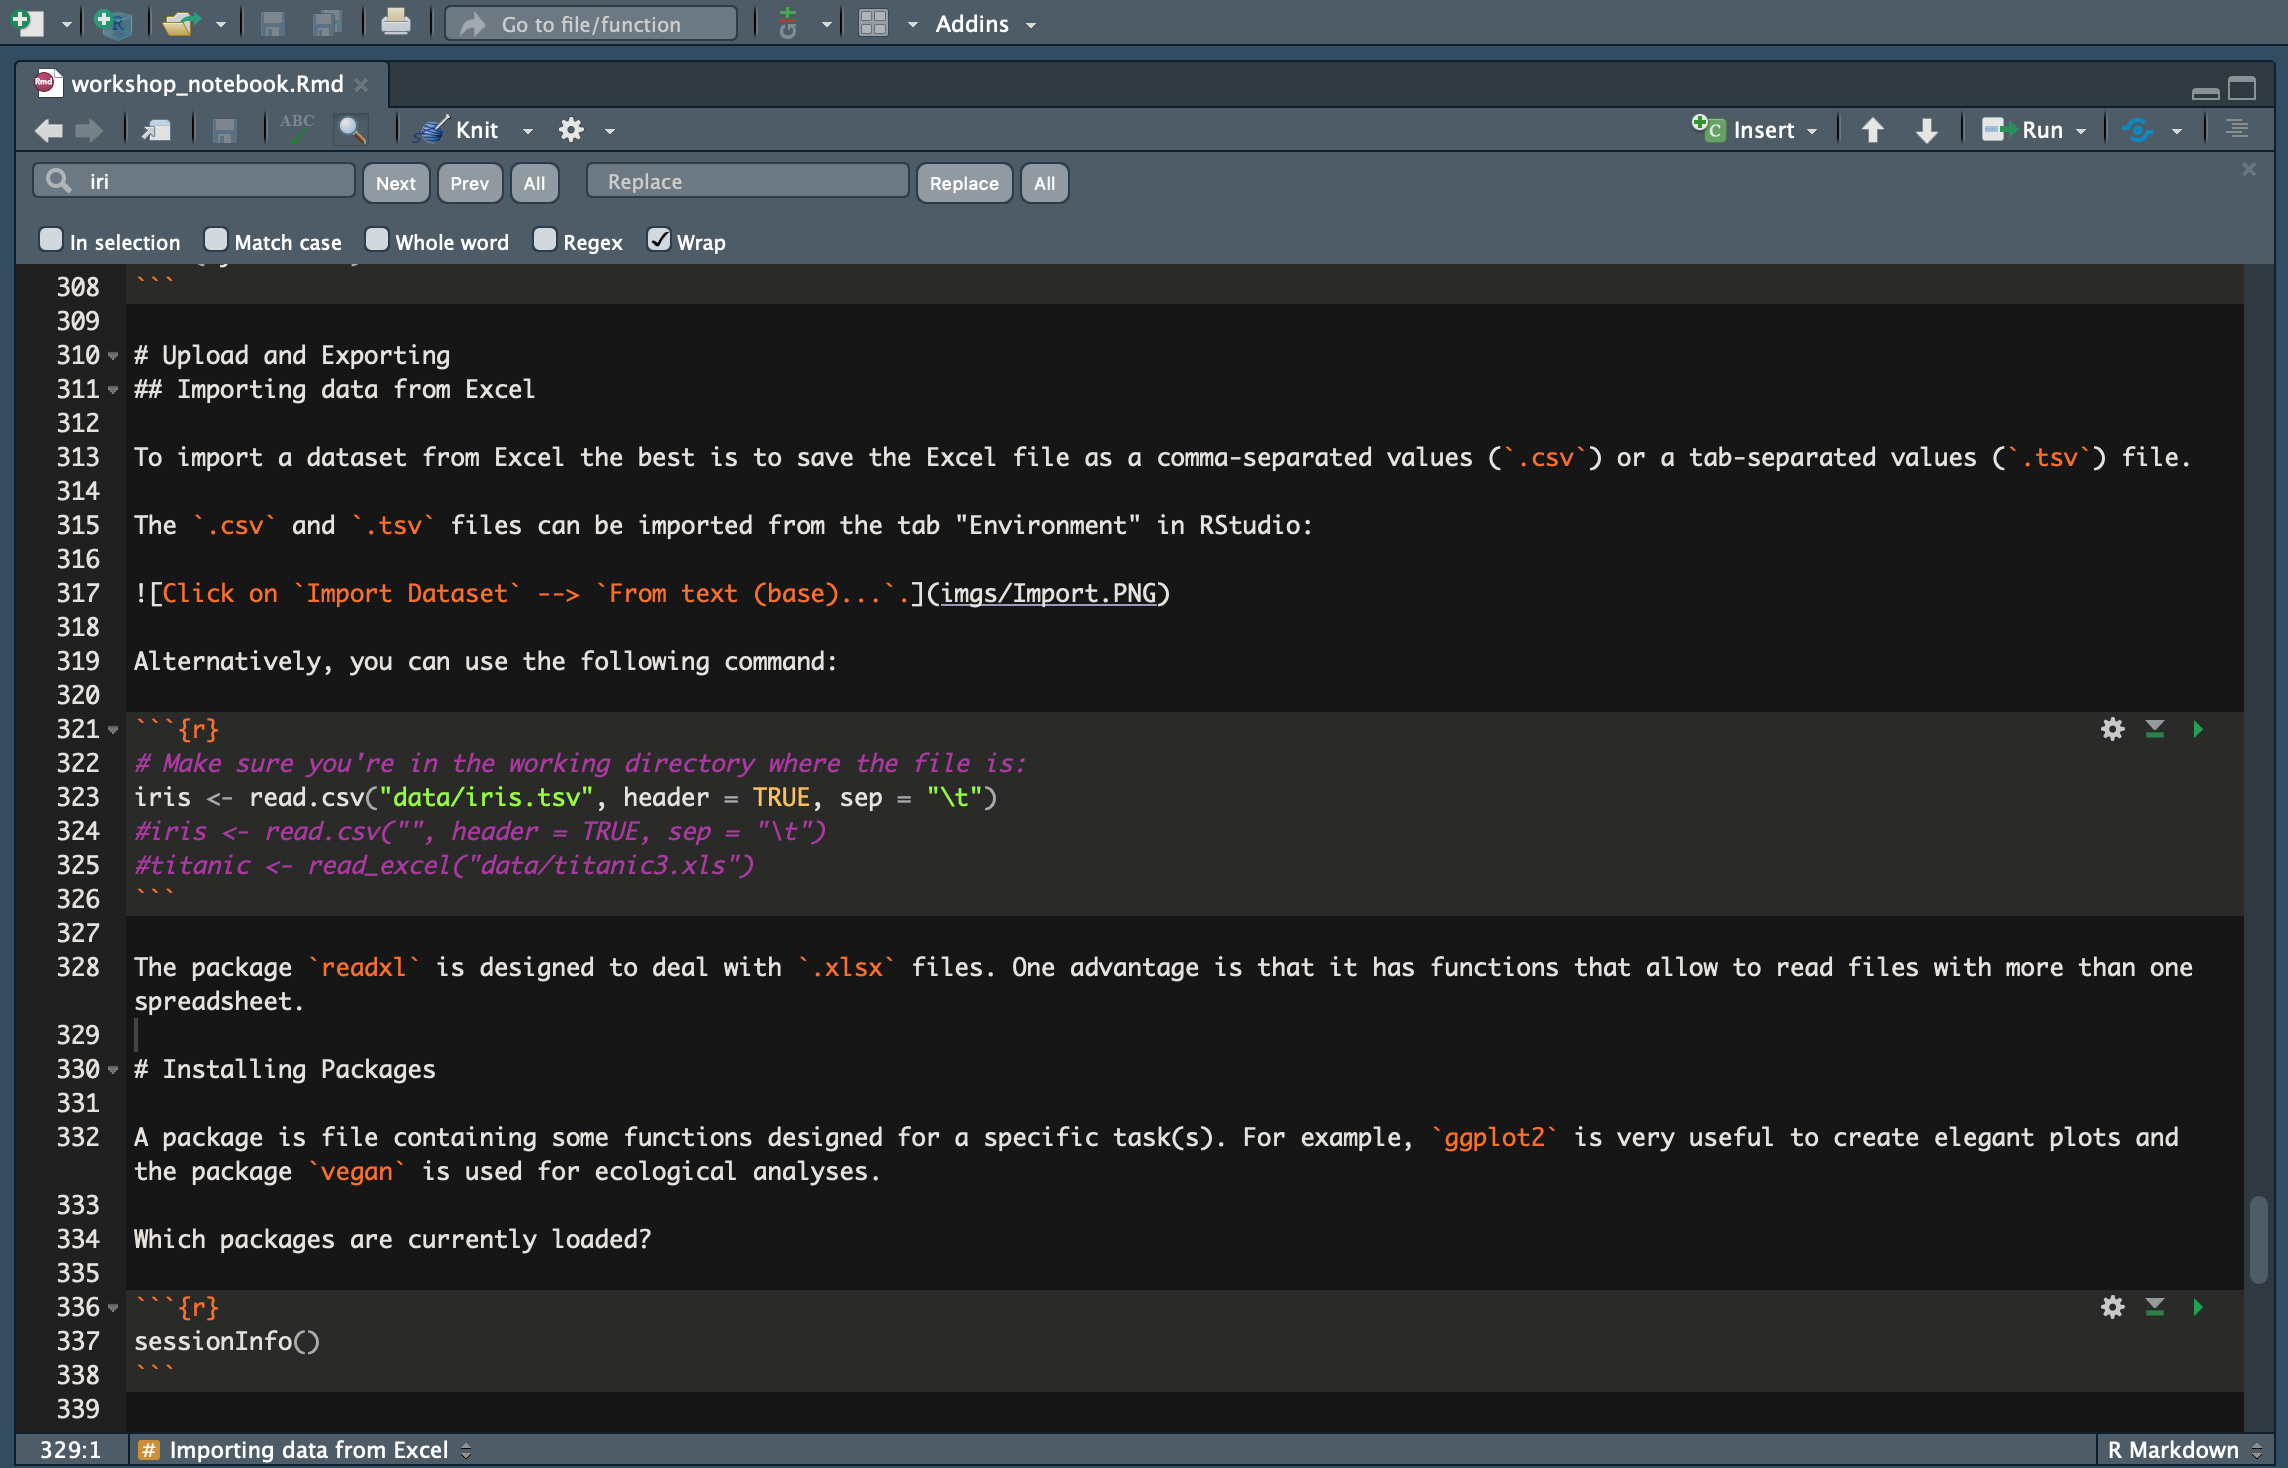
\includegraphics{imgs/1_scripts.png}

\hypertarget{console}{%
\subsubsection{2. Console}\label{console}}

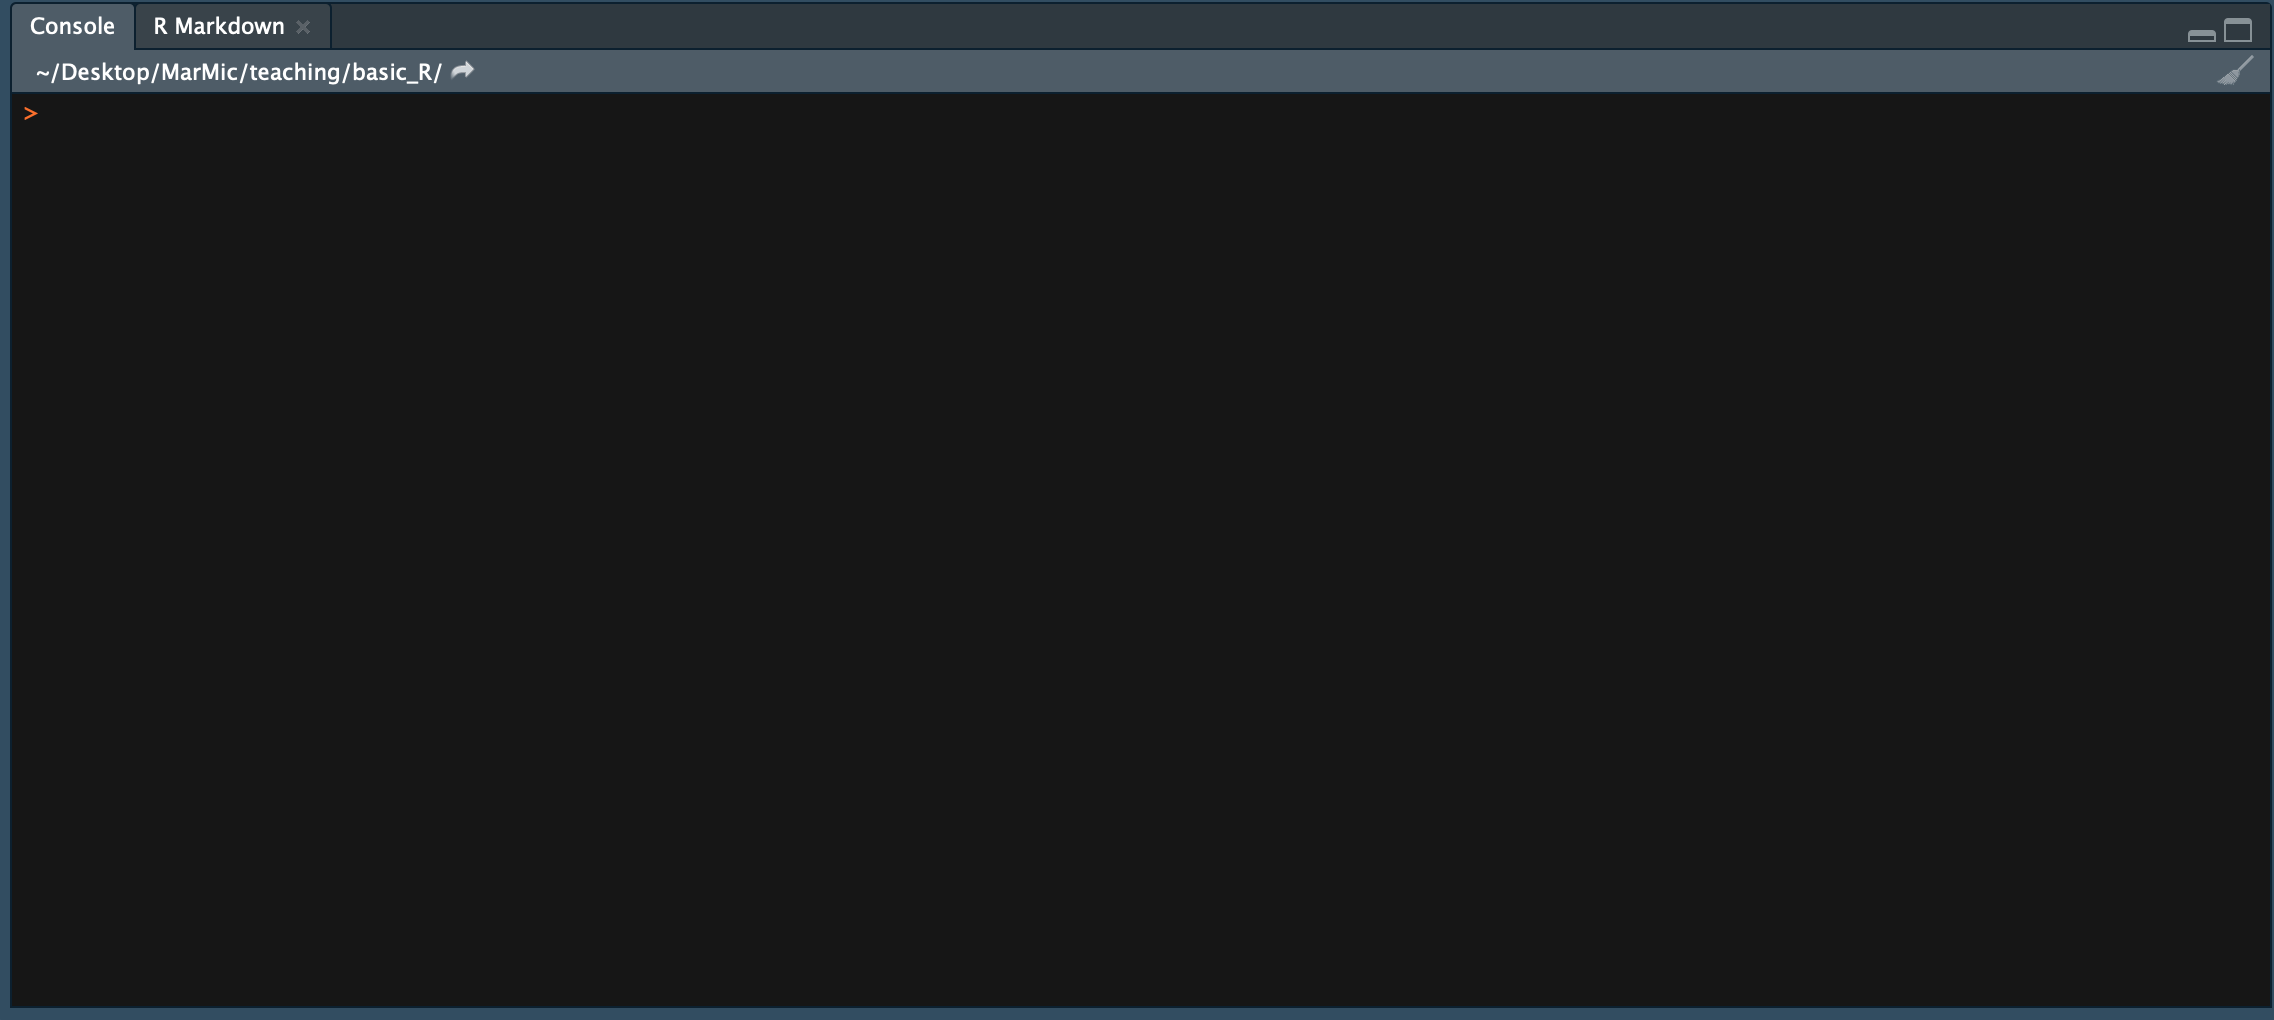
\includegraphics{imgs/2_console.png}

\hypertarget{environment.-where-data-objectsr-objects-are-stored}{%
\subsubsection{3. Environment. Where data objects/R objects are
stored}\label{environment.-where-data-objectsr-objects-are-stored}}

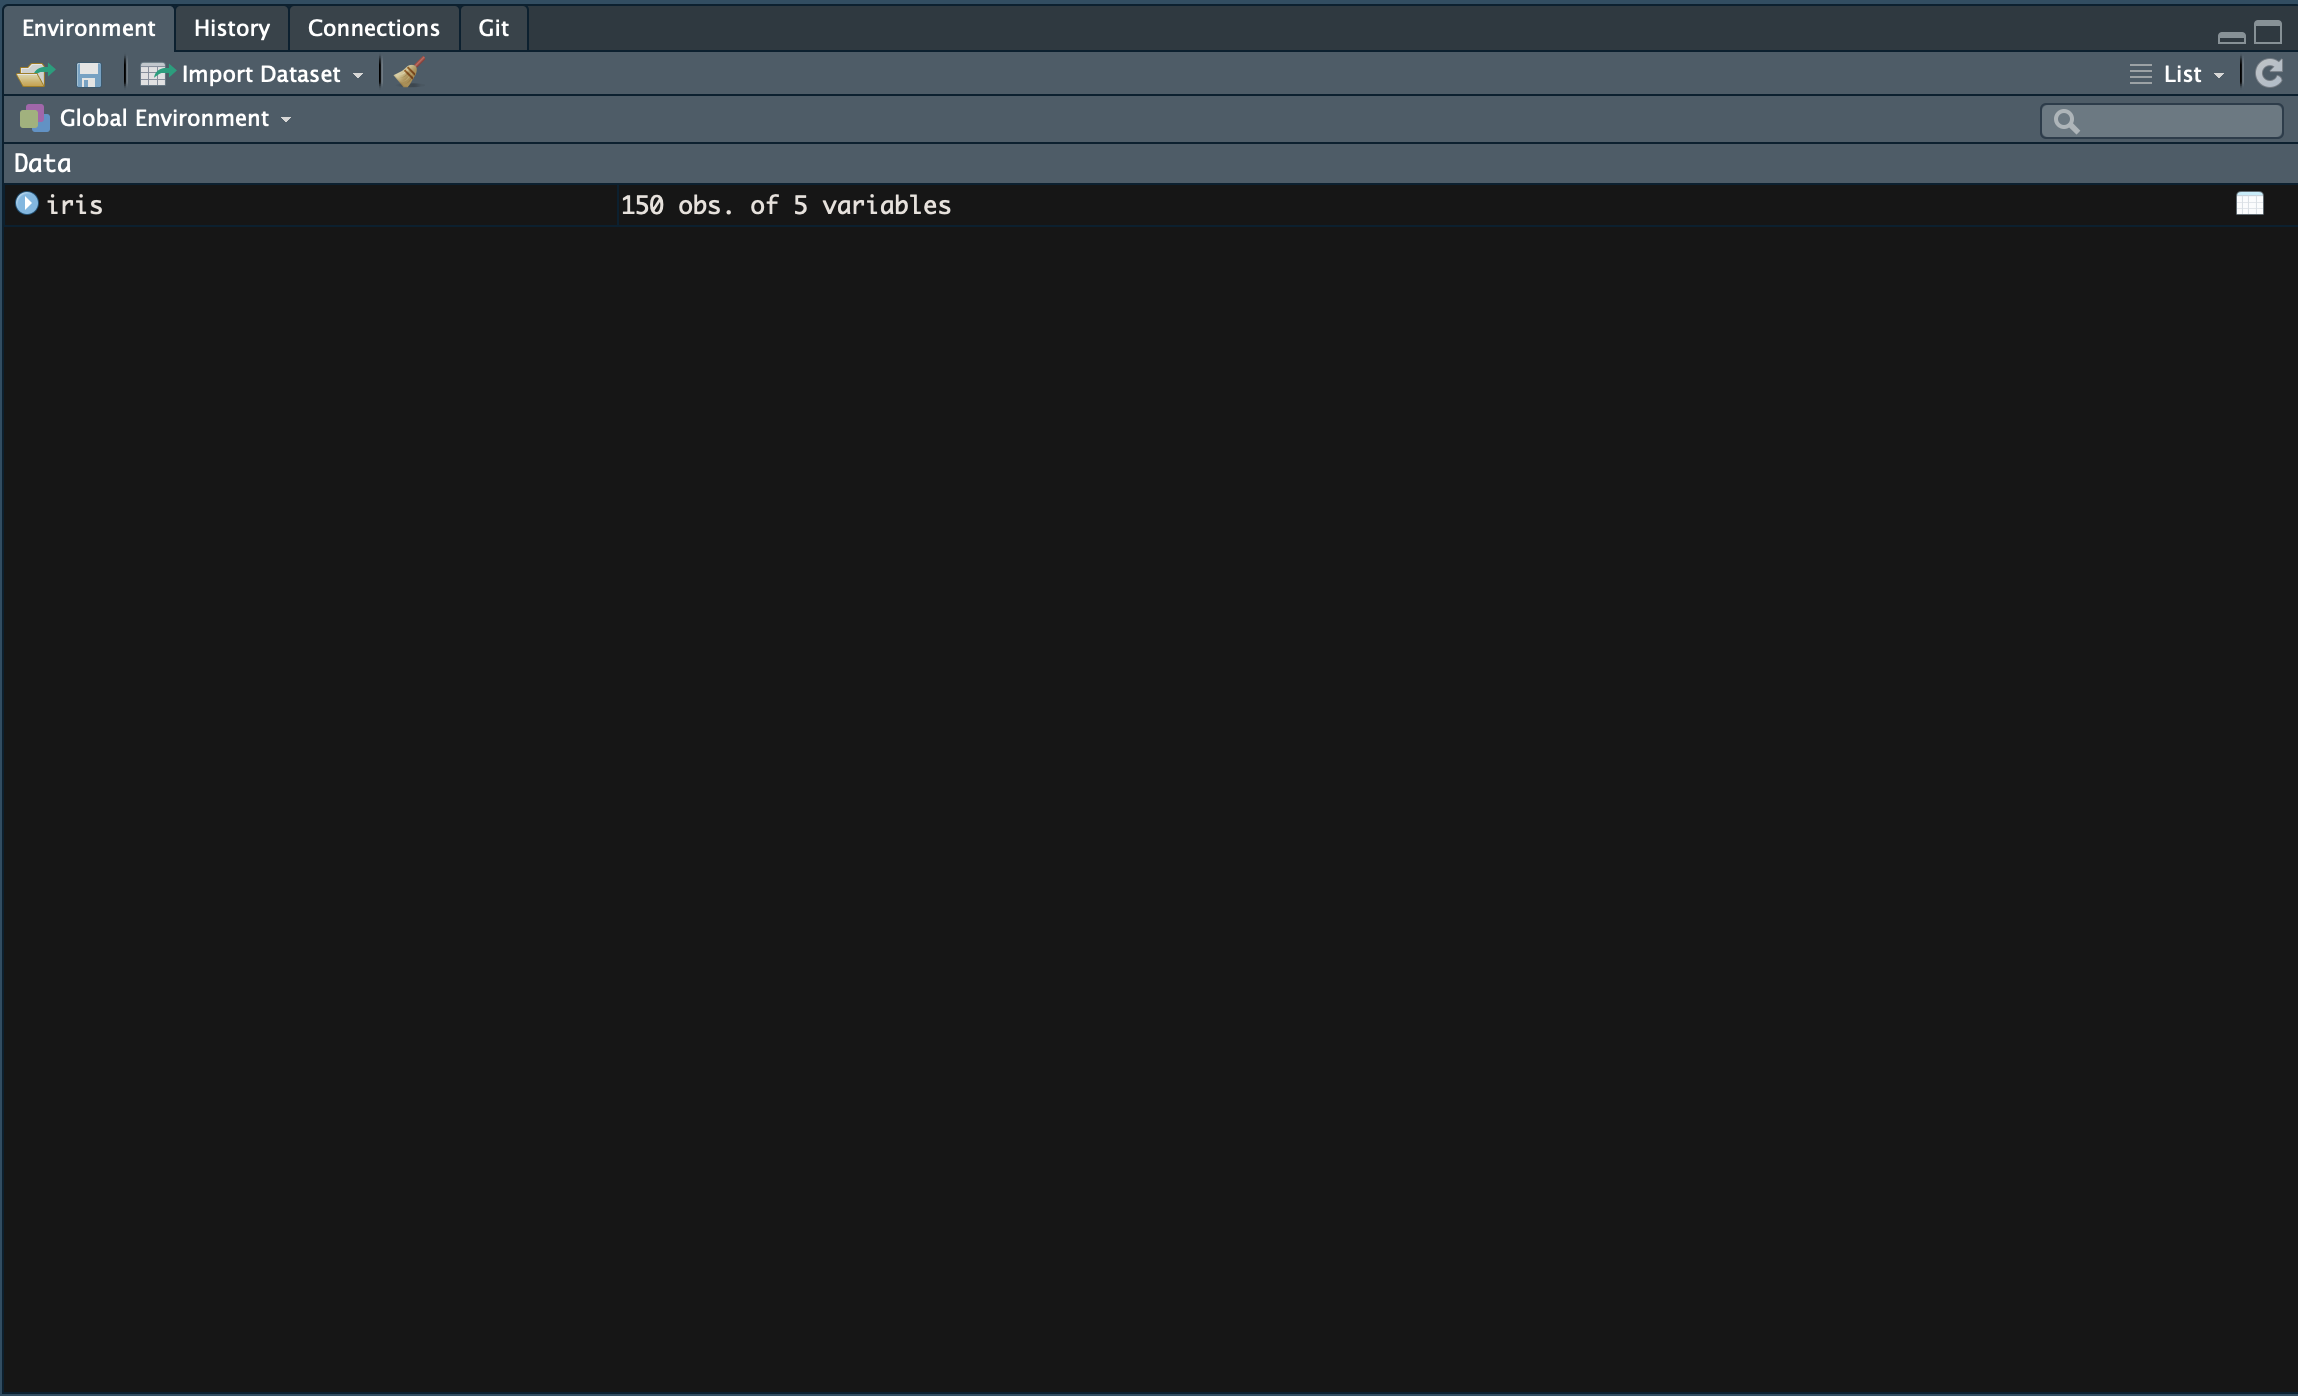
\includegraphics{imgs/3_environment.png}

\hypertarget{plothelpetc-window}{%
\subsubsection{4. Plot/Help/etc window}\label{plothelpetc-window}}

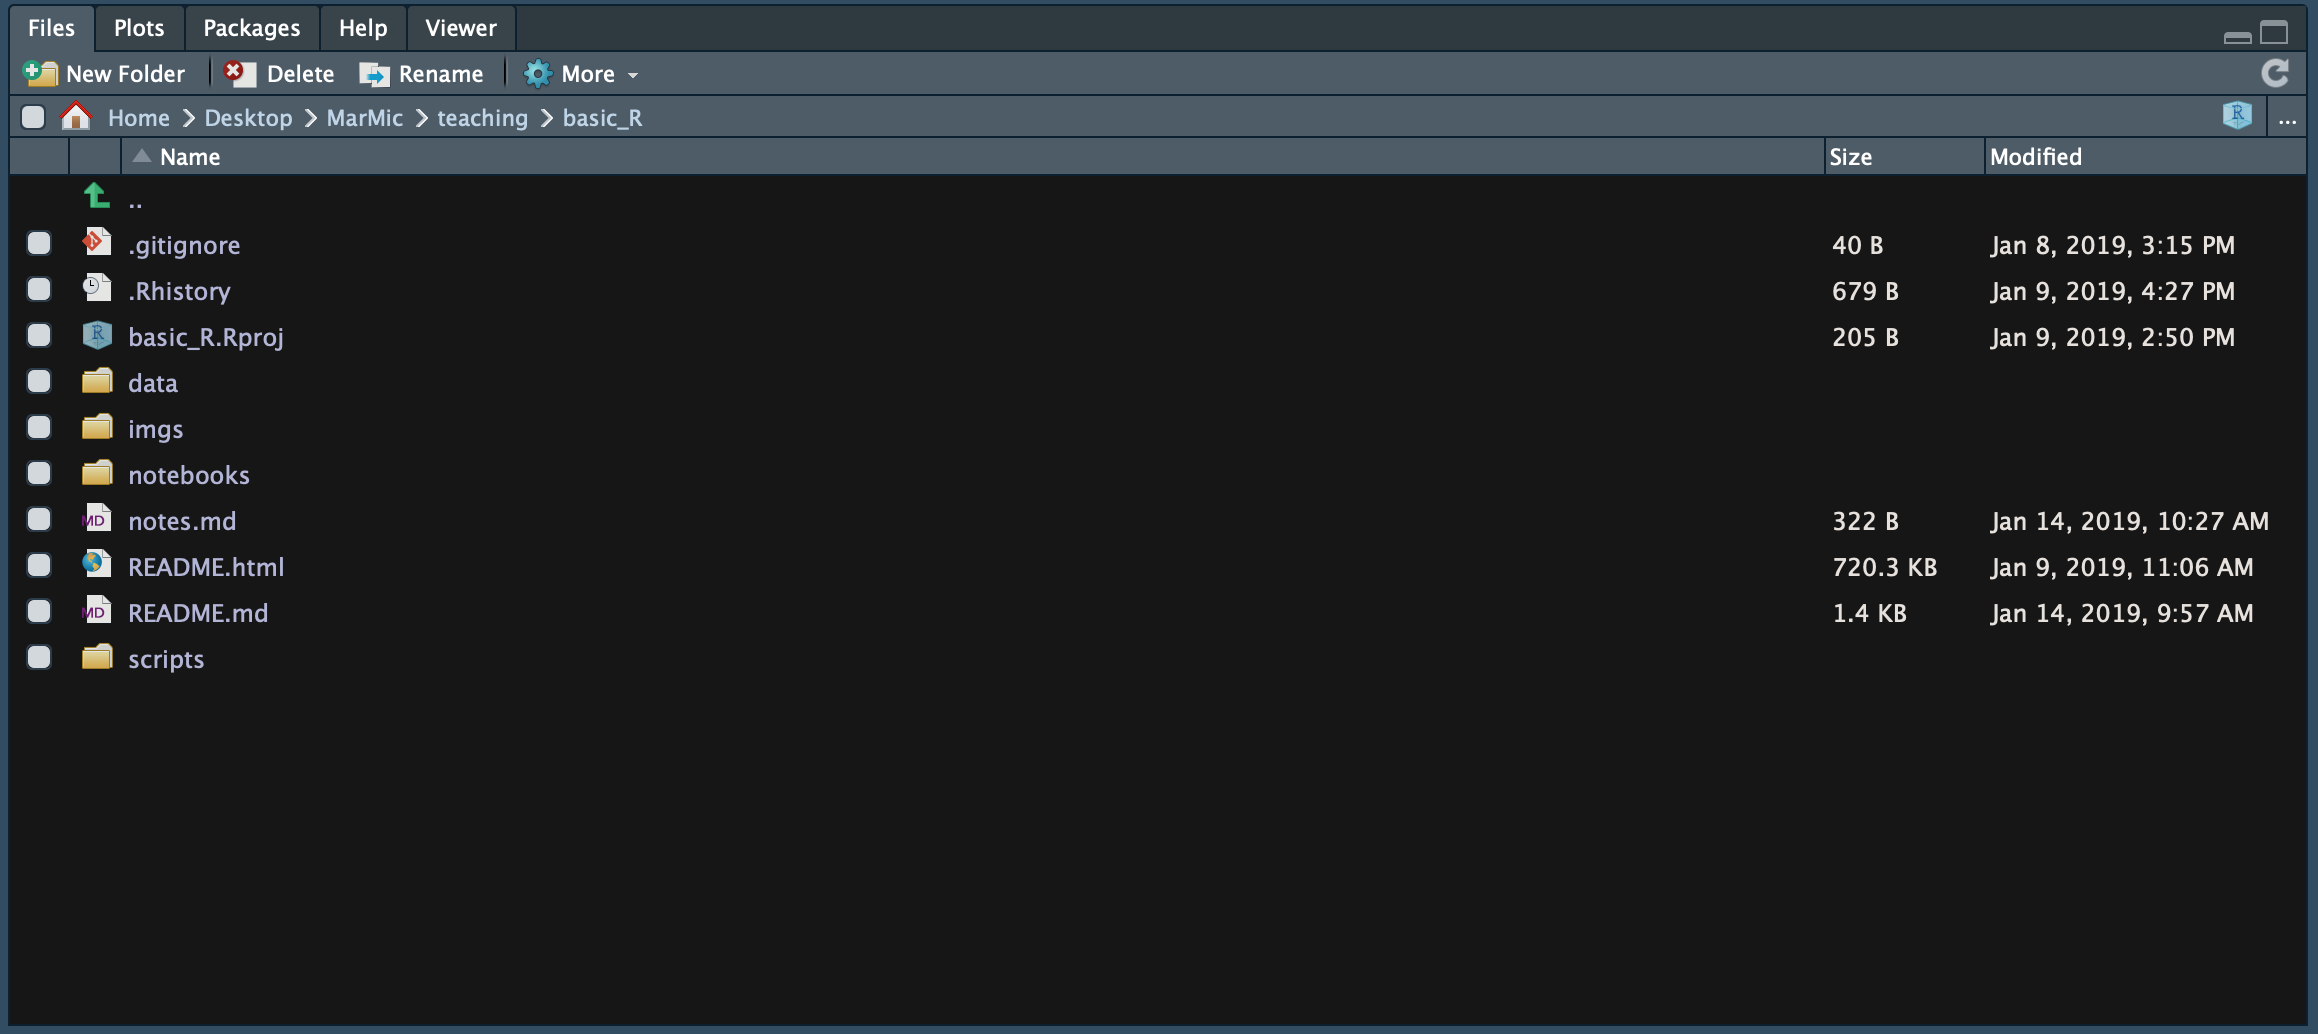
\includegraphics{imgs/4_files.png}

\hypertarget{introduction-to-r-programming-language}{%
\section{Introduction to R programming
language}\label{introduction-to-r-programming-language}}

\begin{center}\rule{0.5\linewidth}{\linethickness}\end{center}

We are getting into the exciting stuff! Open RStudio and start a new R
script. This is like a text file where we will write and execute our
commands.

\hypertarget{intro}{%
\subsection{Intro}\label{intro}}

When writing R code, using hashtags (\#) to include comments is highly
recommended to make the notes understandable. Example:

\begin{Shaded}
\begin{Highlighting}[]
\KeywordTok{print}\NormalTok{(}\StringTok{"Hello"}\NormalTok{) }\CommentTok{# This command prints an initial greeting :)}
\end{Highlighting}
\end{Shaded}

\begin{verbatim}
## [1] "Hello"
\end{verbatim}

\hypertarget{how-to-get-help}{%
\subsection{How to get help}\label{how-to-get-help}}

Use \texttt{?} to read the help page of functions or data sets. For
example:

\texttt{?R.version}

or

\texttt{help(R.Version)}

The \href{https://www.rstudio.com/resources/cheatsheets/}{RStudio
cheatsheets} are a great resource.

Also check \href{https://stackoverflow.com/questions/tagged/r}{Stack
Overflow} frequently :)

\hypertarget{object-names}{%
\subsection{Object names}\label{object-names}}

To assign an object to a name we use \texttt{\textless{}-} (equivalent
to \texttt{=}). The typing shortcut is \texttt{Cntr} + \texttt{-}.
Names\ldots{}

\begin{itemize}
\tightlist
\item
  \ldots{} are case sensitive
\item
  \ldots{} can contain letters, numbers, ``.'' and "\_". They should
  start with a letter.
\item
  \ldots{} should not have function or operator names:
  \texttt{function}, \texttt{if}, \texttt{c}\ldots{}
\end{itemize}

Example:

\begin{Shaded}
\begin{Highlighting}[]
\NormalTok{Greeting <-}\StringTok{ "Hello world!"}

\NormalTok{Greeting}
\end{Highlighting}
\end{Shaded}

\begin{verbatim}
## [1] "Hello world!"
\end{verbatim}

\hypertarget{data-objects}{%
\subsection{Data objects}\label{data-objects}}

There are the following types of objects:

\begin{itemize}
\tightlist
\item
  \textbf{Vectors}
\item
  \textbf{Factors}. For qualitative data.
\item
  \textbf{Lists}. Can contain vectors of different types (integer,
  double, Boolean\ldots).
\item
  \textbf{Arrays}. Vectors organised by rows and columns. It can only
  store data of one type.
\item
  \textbf{Data frames}. Like an array but can contain columns of
  different types. The columns are called \emph{variables}. A data frame
  is the most common way of storing data in R.
\end{itemize}

Some examples:

\begin{Shaded}
\begin{Highlighting}[]
\CommentTok{# Vectors}
\NormalTok{x <-}\StringTok{ }\KeywordTok{c}\NormalTok{(}\DecValTok{8}\NormalTok{,}\DecValTok{2}\NormalTok{,}\DecValTok{5}\NormalTok{,}\DecValTok{6}\NormalTok{,}\DecValTok{7}\NormalTok{)}
\NormalTok{y <-}\StringTok{ }\KeywordTok{c}\NormalTok{(}\DecValTok{34}\NormalTok{,}\DecValTok{23}\NormalTok{,}\DecValTok{67}\NormalTok{,}\DecValTok{65}\NormalTok{,}\DecValTok{23}\NormalTok{)}
\NormalTok{z <-}\StringTok{ }\KeywordTok{c}\NormalTok{(}\OtherTok{TRUE}\NormalTok{, }\OtherTok{TRUE}\NormalTok{, }\OtherTok{FALSE}\NormalTok{, }\OtherTok{FALSE}\NormalTok{, }\OtherTok{TRUE}\NormalTok{)}
\NormalTok{w <-}\StringTok{ }\KeywordTok{c}\NormalTok{(}\StringTok{"Hello"}\NormalTok{, }\StringTok{"Hallo"}\NormalTok{, }\StringTok{"Hola"}\NormalTok{)}

\CommentTok{# Factors}
\NormalTok{a <-}\StringTok{ }\KeywordTok{factor}\NormalTok{(}\KeywordTok{c}\NormalTok{(}\DecValTok{1}\NormalTok{,}\DecValTok{2}\NormalTok{,}\DecValTok{3}\NormalTok{,}\DecValTok{4}\NormalTok{,}\DecValTok{5}\NormalTok{))}
\NormalTok{b <-}\StringTok{ }\KeywordTok{factor}\NormalTok{(}\KeywordTok{c}\NormalTok{(}\StringTok{"a"}\NormalTok{, }\StringTok{"b"}\NormalTok{, }\StringTok{"c"}\NormalTok{, }\StringTok{"d"}\NormalTok{, }\StringTok{"e"}\NormalTok{))}

\CommentTok{# Lists}
\NormalTok{l <-}\StringTok{ }\KeywordTok{list}\NormalTok{(}\DecValTok{1}\OperatorTok{:}\DecValTok{3}\NormalTok{, }\StringTok{"a"}\NormalTok{, }\KeywordTok{c}\NormalTok{(}\OtherTok{TRUE}\NormalTok{, }\OtherTok{FALSE}\NormalTok{, }\OtherTok{TRUE}\NormalTok{), }\KeywordTok{c}\NormalTok{(}\FloatTok{2.3}\NormalTok{, }\FloatTok{5.9}\NormalTok{))}
\NormalTok{l}
\end{Highlighting}
\end{Shaded}

\begin{verbatim}
## [[1]]
## [1] 1 2 3
## 
## [[2]]
## [1] "a"
## 
## [[3]]
## [1]  TRUE FALSE  TRUE
## 
## [[4]]
## [1] 2.3 5.9
\end{verbatim}

\begin{Shaded}
\begin{Highlighting}[]
\CommentTok{# The elements in a list can be named:}
\NormalTok{l_named <-}\StringTok{ }\KeywordTok{list}\NormalTok{(}\DataTypeTok{int =} \DecValTok{1}\OperatorTok{:}\DecValTok{3}\NormalTok{, }\DataTypeTok{char =} \StringTok{"a"}\NormalTok{, }\DataTypeTok{bool =} \KeywordTok{c}\NormalTok{(}\OtherTok{TRUE}\NormalTok{, }\OtherTok{FALSE}\NormalTok{, }\OtherTok{TRUE}\NormalTok{), }\DataTypeTok{dbl =} \KeywordTok{c}\NormalTok{(}\FloatTok{2.3}\NormalTok{, }\FloatTok{5.9}\NormalTok{))}
\NormalTok{l_named}
\end{Highlighting}
\end{Shaded}

\begin{verbatim}
## $int
## [1] 1 2 3
## 
## $char
## [1] "a"
## 
## $bool
## [1]  TRUE FALSE  TRUE
## 
## $dbl
## [1] 2.3 5.9
\end{verbatim}

\begin{Shaded}
\begin{Highlighting}[]
\CommentTok{# Array}
\NormalTok{num.data <-}\StringTok{ }\KeywordTok{array}\NormalTok{(}\KeywordTok{c}\NormalTok{(x, y, z), }\DataTypeTok{dim=}\KeywordTok{c}\NormalTok{(}\DecValTok{5}\NormalTok{,}\DecValTok{3}\NormalTok{))}
\NormalTok{num.data }\CommentTok{# Note that the logical vector is turned into a vector of 0 and 1.}
\end{Highlighting}
\end{Shaded}

\begin{verbatim}
##      [,1] [,2] [,3]
## [1,]    8   34    1
## [2,]    2   23    1
## [3,]    5   67    0
## [4,]    6   65    0
## [5,]    7   23    1
\end{verbatim}

\begin{Shaded}
\begin{Highlighting}[]
\CommentTok{# You can also transpose an array:}
\NormalTok{num.data.t <-}\StringTok{ }\KeywordTok{t}\NormalTok{(num.data)}
\NormalTok{num.data.t}
\end{Highlighting}
\end{Shaded}

\begin{verbatim}
##      [,1] [,2] [,3] [,4] [,5]
## [1,]    8    2    5    6    7
## [2,]   34   23   67   65   23
## [3,]    1    1    0    0    1
\end{verbatim}

\begin{Shaded}
\begin{Highlighting}[]
\CommentTok{# Data frame}
\NormalTok{my.data <-}\StringTok{ }\KeywordTok{data.frame}\NormalTok{(num.data, }\DataTypeTok{row.names =}\NormalTok{ b)}
\NormalTok{my.data}
\end{Highlighting}
\end{Shaded}

\begin{verbatim}
##   X1 X2 X3
## a  8 34  1
## b  2 23  1
## c  5 67  0
## d  6 65  0
## e  7 23  1
\end{verbatim}

\begin{Shaded}
\begin{Highlighting}[]
\CommentTok{# You can also create your data frame in a more organised way:}
\NormalTok{my.data.org <-}\StringTok{ }\KeywordTok{data.frame}\NormalTok{(x, y, z, }\DataTypeTok{row.names =}\NormalTok{ b)}
\NormalTok{my.data.org}
\end{Highlighting}
\end{Shaded}

\begin{verbatim}
##   x  y     z
## a 8 34  TRUE
## b 2 23  TRUE
## c 5 67 FALSE
## d 6 65 FALSE
## e 7 23  TRUE
\end{verbatim}

\textbf{YOUR TURN \#1} - Make an R object with the names of your best
friends and print it.

\hypertarget{attributes-of-the-objects-and-their-functions}{%
\subsection{Attributes of the objects and their
functions}\label{attributes-of-the-objects-and-their-functions}}

\begin{itemize}
\tightlist
\item
  Attributes \texttt{attributes}
\item
  Mode \texttt{mode}
\item
  Type \texttt{typeof}
\item
  Names \texttt{names}
\item
  Dimensions \texttt{dim}. Only in two-dimensional data.
\item
  Names of the dimensions \texttt{dimnames}
\item
  Class \texttt{class}
\end{itemize}

Check what are the attributes of the objects created before. For
example:

\begin{Shaded}
\begin{Highlighting}[]
\KeywordTok{dim}\NormalTok{(x)}
\end{Highlighting}
\end{Shaded}

\begin{verbatim}
## NULL
\end{verbatim}

\begin{Shaded}
\begin{Highlighting}[]
\KeywordTok{dim}\NormalTok{(my.data)}
\end{Highlighting}
\end{Shaded}

\begin{verbatim}
## [1] 5 3
\end{verbatim}

\begin{Shaded}
\begin{Highlighting}[]
\KeywordTok{dimnames}\NormalTok{(my.data)}
\end{Highlighting}
\end{Shaded}

\begin{verbatim}
## [[1]]
## [1] "a" "b" "c" "d" "e"
## 
## [[2]]
## [1] "X1" "X2" "X3"
\end{verbatim}

\begin{Shaded}
\begin{Highlighting}[]
\KeywordTok{attributes}\NormalTok{(my.data.org)}
\end{Highlighting}
\end{Shaded}

\begin{verbatim}
## $names
## [1] "x" "y" "z"
## 
## $class
## [1] "data.frame"
## 
## $row.names
## [1] "a" "b" "c" "d" "e"
\end{verbatim}

\begin{Shaded}
\begin{Highlighting}[]
\CommentTok{# etc}
\end{Highlighting}
\end{Shaded}

\textbf{YOUR TURN \#2} - Create a data frame containing some information
about these friends: the row names are the names of your friends, the
first column is their age, the second column is their hair colour and
the third column is\ldots{} you choose! Explore the attributes,
dimensions, dimension names, etc. of this data frame.

\hypertarget{basic-maths-and-statistics-in-r}{%
\subsection{Basic maths and statistics in
R}\label{basic-maths-and-statistics-in-r}}

\begin{itemize}
\tightlist
\item
  \texttt{+}, \texttt{-}, \texttt{*} and \texttt{/}
\item
  \texttt{\^{}} and \texttt{sqrt}
\item
  \texttt{exp}, \texttt{log}, \texttt{log10}, \texttt{log2},
  \texttt{logb(x,\ base)}
\item
  \texttt{max}, \texttt{min}, \texttt{range}, \texttt{mean},
  \texttt{median}, \texttt{var}, \texttt{sd}, \texttt{quantile},
  \texttt{sum}\ldots{}
\item
  Logical operators: \texttt{\textless{}}, \texttt{\textless{}=},
  \texttt{\textgreater{}}, \texttt{\textgreater{}=}, \texttt{==}
  (\emph{equals}), \texttt{!=} (\emph{not equal to}), \texttt{\&\&}
  (\emph{and}), \texttt{\textbar{}\textbar{}} (\emph{or}).
\item
  Logical clauses \texttt{if()\ \{\}\ else\ \{\}}.
\item
  Set operations: \texttt{union(x,\ y)},
  \texttt{intersect(x,\ y)}\ldots{}
\end{itemize}

Examples:

\begin{Shaded}
\begin{Highlighting}[]
\NormalTok{x}\OperatorTok{^}\DecValTok{2}
\end{Highlighting}
\end{Shaded}

\begin{verbatim}
## [1] 64  4 25 36 49
\end{verbatim}

\begin{Shaded}
\begin{Highlighting}[]
\NormalTok{x}\OperatorTok{+}\NormalTok{y}
\end{Highlighting}
\end{Shaded}

\begin{verbatim}
## [1] 42 25 72 71 30
\end{verbatim}

\begin{Shaded}
\begin{Highlighting}[]
\KeywordTok{sum}\NormalTok{(x)}
\end{Highlighting}
\end{Shaded}

\begin{verbatim}
## [1] 28
\end{verbatim}

\begin{Shaded}
\begin{Highlighting}[]
\KeywordTok{mean}\NormalTok{(x)}
\end{Highlighting}
\end{Shaded}

\begin{verbatim}
## [1] 5.6
\end{verbatim}

\begin{Shaded}
\begin{Highlighting}[]
\KeywordTok{median}\NormalTok{(x)}
\end{Highlighting}
\end{Shaded}

\begin{verbatim}
## [1] 6
\end{verbatim}

\begin{Shaded}
\begin{Highlighting}[]
\KeywordTok{var}\NormalTok{(x)}
\end{Highlighting}
\end{Shaded}

\begin{verbatim}
## [1] 5.3
\end{verbatim}

\begin{Shaded}
\begin{Highlighting}[]
\NormalTok{x }\OperatorTok{>}\StringTok{ }\DecValTok{5}
\end{Highlighting}
\end{Shaded}

\begin{verbatim}
## [1]  TRUE FALSE FALSE  TRUE  TRUE
\end{verbatim}

\begin{Shaded}
\begin{Highlighting}[]
\NormalTok{x }\OperatorTok{>=}\StringTok{ }\DecValTok{5}
\end{Highlighting}
\end{Shaded}

\begin{verbatim}
## [1]  TRUE FALSE  TRUE  TRUE  TRUE
\end{verbatim}

\begin{Shaded}
\begin{Highlighting}[]
\NormalTok{x }\OperatorTok{==}\StringTok{ }\DecValTok{5}
\end{Highlighting}
\end{Shaded}

\begin{verbatim}
## [1] FALSE FALSE  TRUE FALSE FALSE
\end{verbatim}

\begin{Shaded}
\begin{Highlighting}[]
\ControlFlowTok{if}\NormalTok{(}\KeywordTok{min}\NormalTok{(x)}\OperatorTok{>}\DecValTok{1} \OperatorTok{&&}\StringTok{ }\KeywordTok{min}\NormalTok{(y)}\OperatorTok{<}\DecValTok{10}\NormalTok{) \{}
  \KeywordTok{print}\NormalTok{(}\StringTok{"Yes"}\NormalTok{)}
\NormalTok{\} }\ControlFlowTok{else}\NormalTok{ \{}
  \KeywordTok{print}\NormalTok{(}\StringTok{"No"}\NormalTok{)}
\NormalTok{\}}
\end{Highlighting}
\end{Shaded}

\begin{verbatim}
## [1] "No"
\end{verbatim}

\begin{Shaded}
\begin{Highlighting}[]
\ControlFlowTok{if}\NormalTok{(}\KeywordTok{min}\NormalTok{(x)}\OperatorTok{>}\DecValTok{1} \OperatorTok{||}\StringTok{ }\KeywordTok{min}\NormalTok{(y)}\OperatorTok{<}\DecValTok{10}\NormalTok{) \{}
  \KeywordTok{print}\NormalTok{(}\StringTok{"Yes"}\NormalTok{)}
\NormalTok{\} }\ControlFlowTok{else}\NormalTok{ \{}
  \KeywordTok{print}\NormalTok{(}\StringTok{"No"}\NormalTok{)}
\NormalTok{\}}
\end{Highlighting}
\end{Shaded}

\begin{verbatim}
## [1] "Yes"
\end{verbatim}

\hypertarget{subsetting-strings-and-arrays}{%
\subsection{Subsetting strings and
arrays}\label{subsetting-strings-and-arrays}}

With the function \texttt{c()} we can generate \textbf{strings} of
values. With the coordinates (square brackets, \texttt{{[}} and
\texttt{{]}}) we can \textbf{select} specific elements from strings.
With the operator \texttt{\$} we can access columns in a \textbf{data
frame} by the variable name. For \emph{lists} we can use the operators
\texttt{{[}\ {]}}, that will return a list, or \texttt{{[}{[}\ {]}{]}}
that will return the elements of the list

You can find some help on subsetting
\href{http://www.statmethods.net/management/subset.html}{here} and
\href{http://adv-r.had.co.nz/Subsetting.html}{here}

Examples:

\begin{Shaded}
\begin{Highlighting}[]
\CommentTok{# Generate a vector of consecutive numbers:}
\NormalTok{g <-}\StringTok{ }\KeywordTok{c}\NormalTok{(}\DecValTok{1}\OperatorTok{:}\DecValTok{7}\NormalTok{)}
\NormalTok{g}
\end{Highlighting}
\end{Shaded}

\begin{verbatim}
## [1] 1 2 3 4 5 6 7
\end{verbatim}

\begin{Shaded}
\begin{Highlighting}[]
\CommentTok{# Generate vectors of repeated values:}
\NormalTok{h <-}\StringTok{ }\KeywordTok{rep}\NormalTok{(}\DecValTok{4}\NormalTok{, }\DataTypeTok{times=}\DecValTok{7}\NormalTok{)}
\NormalTok{h}
\end{Highlighting}
\end{Shaded}

\begin{verbatim}
## [1] 4 4 4 4 4 4 4
\end{verbatim}

\begin{Shaded}
\begin{Highlighting}[]
\CommentTok{# Select specific elements from a vector}
\NormalTok{x}
\end{Highlighting}
\end{Shaded}

\begin{verbatim}
## [1] 8 2 5 6 7
\end{verbatim}

\begin{Shaded}
\begin{Highlighting}[]
\NormalTok{x[}\DecValTok{2}\NormalTok{]}
\end{Highlighting}
\end{Shaded}

\begin{verbatim}
## [1] 2
\end{verbatim}

\begin{Shaded}
\begin{Highlighting}[]
\NormalTok{x[}\KeywordTok{c}\NormalTok{(}\DecValTok{2}\NormalTok{,}\DecValTok{4}\NormalTok{)]}
\end{Highlighting}
\end{Shaded}

\begin{verbatim}
## [1] 2 6
\end{verbatim}

\begin{Shaded}
\begin{Highlighting}[]
\NormalTok{x[}\DecValTok{2}\OperatorTok{:}\DecValTok{4}\NormalTok{]}
\end{Highlighting}
\end{Shaded}

\begin{verbatim}
## [1] 2 5 6
\end{verbatim}

\begin{Shaded}
\begin{Highlighting}[]
\CommentTok{# Select specific elements from a list}
\NormalTok{l}
\end{Highlighting}
\end{Shaded}

\begin{verbatim}
## [[1]]
## [1] 1 2 3
## 
## [[2]]
## [1] "a"
## 
## [[3]]
## [1]  TRUE FALSE  TRUE
## 
## [[4]]
## [1] 2.3 5.9
\end{verbatim}

\begin{Shaded}
\begin{Highlighting}[]
\NormalTok{l[[}\DecValTok{3}\NormalTok{]]}
\end{Highlighting}
\end{Shaded}

\begin{verbatim}
## [1]  TRUE FALSE  TRUE
\end{verbatim}

\begin{Shaded}
\begin{Highlighting}[]
\NormalTok{l_named}
\end{Highlighting}
\end{Shaded}

\begin{verbatim}
## $int
## [1] 1 2 3
## 
## $char
## [1] "a"
## 
## $bool
## [1]  TRUE FALSE  TRUE
## 
## $dbl
## [1] 2.3 5.9
\end{verbatim}

\begin{Shaded}
\begin{Highlighting}[]
\NormalTok{l_named[[}\DecValTok{3}\NormalTok{]]}
\end{Highlighting}
\end{Shaded}

\begin{verbatim}
## [1]  TRUE FALSE  TRUE
\end{verbatim}

\begin{Shaded}
\begin{Highlighting}[]
\NormalTok{l_named}\OperatorTok{$}\NormalTok{bool }\CommentTok{# If we give names to the items in a list, we can access them with the dolar sign.}
\end{Highlighting}
\end{Shaded}

\begin{verbatim}
## [1]  TRUE FALSE  TRUE
\end{verbatim}

\begin{Shaded}
\begin{Highlighting}[]
\CommentTok{# Select specific elements from a matrix.}
\NormalTok{num.data}
\end{Highlighting}
\end{Shaded}

\begin{verbatim}
##      [,1] [,2] [,3]
## [1,]    8   34    1
## [2,]    2   23    1
## [3,]    5   67    0
## [4,]    6   65    0
## [5,]    7   23    1
\end{verbatim}

\begin{Shaded}
\begin{Highlighting}[]
\NormalTok{num.data[}\DecValTok{1}\NormalTok{, }\DecValTok{1}\NormalTok{]}
\end{Highlighting}
\end{Shaded}

\begin{verbatim}
## [1] 8
\end{verbatim}

\begin{Shaded}
\begin{Highlighting}[]
\NormalTok{num.data[}\DecValTok{1}\OperatorTok{:}\DecValTok{3}\NormalTok{, }\KeywordTok{c}\NormalTok{(}\DecValTok{1}\NormalTok{,}\DecValTok{3}\NormalTok{)]}
\end{Highlighting}
\end{Shaded}

\begin{verbatim}
##      [,1] [,2]
## [1,]    8    1
## [2,]    2    1
## [3,]    5    0
\end{verbatim}

\begin{Shaded}
\begin{Highlighting}[]
\CommentTok{# This is useful to make subsets:}
\NormalTok{num.data.subset <-}\StringTok{ }\NormalTok{num.data[,}\DecValTok{1}\OperatorTok{:}\DecValTok{2}\NormalTok{]}
\NormalTok{num.data.subset}
\end{Highlighting}
\end{Shaded}

\begin{verbatim}
##      [,1] [,2]
## [1,]    8   34
## [2,]    2   23
## [3,]    5   67
## [4,]    6   65
## [5,]    7   23
\end{verbatim}

\begin{Shaded}
\begin{Highlighting}[]
\CommentTok{# Select elements using conditionals:}
\NormalTok{g[g }\OperatorTok{>}\StringTok{ }\DecValTok{4}\NormalTok{]}
\end{Highlighting}
\end{Shaded}

\begin{verbatim}
## [1] 5 6 7
\end{verbatim}

\begin{Shaded}
\begin{Highlighting}[]
\NormalTok{g[g }\OperatorTok{>=}\StringTok{ }\DecValTok{4}\NormalTok{]}
\end{Highlighting}
\end{Shaded}

\begin{verbatim}
## [1] 4 5 6 7
\end{verbatim}

\begin{Shaded}
\begin{Highlighting}[]
\CommentTok{# You can also select strings of letters}
\NormalTok{my.letters <-}\StringTok{ }\NormalTok{letters[}\DecValTok{1}\OperatorTok{:}\DecValTok{6}\NormalTok{]}
\NormalTok{my.letters}
\end{Highlighting}
\end{Shaded}

\begin{verbatim}
## [1] "a" "b" "c" "d" "e" "f"
\end{verbatim}

\begin{Shaded}
\begin{Highlighting}[]
\CommentTok{# Also capital letters.}
\NormalTok{MY.LETTERS <-}\StringTok{ }\NormalTok{LETTERS[}\DecValTok{1}\OperatorTok{:}\DecValTok{6}\NormalTok{]}
\NormalTok{MY.LETTERS}
\end{Highlighting}
\end{Shaded}

\begin{verbatim}
## [1] "A" "B" "C" "D" "E" "F"
\end{verbatim}

\begin{Shaded}
\begin{Highlighting}[]
\CommentTok{# Access the variables in a data frame.}
\NormalTok{my.data.org}\OperatorTok{$}\NormalTok{x}
\end{Highlighting}
\end{Shaded}

\begin{verbatim}
## [1] 8 2 5 6 7
\end{verbatim}

\begin{Shaded}
\begin{Highlighting}[]
\NormalTok{my.data.org}\OperatorTok{$}\NormalTok{y}
\end{Highlighting}
\end{Shaded}

\begin{verbatim}
## [1] 34 23 67 65 23
\end{verbatim}

\textbf{YOUR TURN \#3} - You've decided you're not friends with one of
people in the \texttt{friends} data frame. You want to remove his/her
information from your data frame.

\textbf{YOUR TURN \#4} - Select the friends from the dataframe that are
older than 27.

\hypertarget{generate-random-sequences}{%
\subsubsection{Generate random
sequences}\label{generate-random-sequences}}

\begin{itemize}
\tightlist
\item
  Check \texttt{?sample}
\end{itemize}

\begin{Shaded}
\begin{Highlighting}[]
\KeywordTok{sample}\NormalTok{(}\DecValTok{10}\NormalTok{)}
\end{Highlighting}
\end{Shaded}

\begin{verbatim}
##  [1] 10  7  9  3  8  2  5  1  6  4
\end{verbatim}

\begin{Shaded}
\begin{Highlighting}[]
\KeywordTok{sample}\NormalTok{(}\DecValTok{10}\NormalTok{, }\DecValTok{4}\NormalTok{)}
\end{Highlighting}
\end{Shaded}

\begin{verbatim}
## [1]  1  7 10  2
\end{verbatim}

\begin{Shaded}
\begin{Highlighting}[]
\KeywordTok{sample}\NormalTok{(}\DecValTok{10}\NormalTok{, }\DataTypeTok{replace=}\OtherTok{TRUE}\NormalTok{)}
\end{Highlighting}
\end{Shaded}

\begin{verbatim}
##  [1] 2 1 3 2 3 5 6 5 8 1
\end{verbatim}

\begin{Shaded}
\begin{Highlighting}[]
\KeywordTok{sample}\NormalTok{(x, }\DataTypeTok{prob=}\NormalTok{(x}\OperatorTok{/}\KeywordTok{sum}\NormalTok{(x)))}
\end{Highlighting}
\end{Shaded}

\begin{verbatim}
## [1] 5 6 7 2 8
\end{verbatim}

\begin{Shaded}
\begin{Highlighting}[]
\KeywordTok{sample}\NormalTok{(x, }\DecValTok{10}\NormalTok{, }\DataTypeTok{replace=}\NormalTok{T, }\DataTypeTok{prob=}\NormalTok{(x}\OperatorTok{/}\KeywordTok{sum}\NormalTok{(x)))}
\end{Highlighting}
\end{Shaded}

\begin{verbatim}
##  [1] 8 8 6 6 5 7 7 8 8 8
\end{verbatim}

\begin{itemize}
\tightlist
\item
  Random distributions. In general, \texttt{rDistribution} generates a
  random distribution with a given sample size (first argument) and
  given parameters. Examples:

  \begin{itemize}
  \tightlist
  \item
    Normal distribution \texttt{rnorm}
  \item
    Student \(t\) distribution \texttt{rt}
  \item
    Poisson distribution \texttt{rpois}
  \item
    \(\chi ^2\) distribution \texttt{rchisq}
  \end{itemize}
\end{itemize}

To visualize it in a histogram:

\begin{Shaded}
\begin{Highlighting}[]
\KeywordTok{rnorm}\NormalTok{(}\DecValTok{100}\NormalTok{, }\DataTypeTok{mean=}\DecValTok{0}\NormalTok{, }\DataTypeTok{sd=}\DecValTok{1}\NormalTok{)}
\end{Highlighting}
\end{Shaded}

\begin{verbatim}
##   [1] -0.841210800 -0.959519067 -0.549570393 -0.655520925  0.809092945
##   [6] -0.297812892 -1.561026359 -1.589925430  1.355298659  1.470567939
##  [11]  0.589575121 -0.708340043 -0.688381678 -0.328393501 -0.294117110
##  [16]  0.601788419 -0.207693770 -0.131079606  0.664131841  0.354846984
##  [21] -0.001181079 -0.229879998  1.098620971 -1.012010231 -0.393399520
##  [26]  0.796916644 -0.272016065 -0.203046919  0.814654310 -0.838122895
##  [31] -0.452189687 -1.305770393 -1.056701687  0.243430822  0.733233560
##  [36]  0.764934518  1.138543096  0.656970288 -0.651291477 -0.194594909
##  [41] -0.101797605  0.419930762  2.387476965  0.331707831 -1.781161333
##  [46]  1.519484470  0.150844250  0.073741967  0.411568868  0.525929782
##  [51] -0.434472942  0.139324924  0.281875804  1.065264984 -1.604925230
##  [56] -0.188621388 -0.221453675 -1.644257588 -1.646682712 -2.106844321
##  [61]  1.317910638  0.971000733 -0.199859296 -0.315999934 -0.559739808
##  [66] -0.778689161 -1.001691275 -0.124571732 -0.346902951  0.069231438
##  [71] -0.238543636  0.949622658  0.403775975  1.367693051 -1.241338002
##  [76] -1.888395195  0.484606692 -0.071353298 -0.884319583 -0.419693581
##  [81] -2.032202918 -0.331907882 -0.742806613 -0.435989408 -0.613598614
##  [86]  0.951864885 -1.477482826  0.937236325 -2.277724505 -0.499712548
##  [91] -0.672144999  0.864684706  0.592472775 -0.172417695 -1.846006837
##  [96] -0.078904680 -0.339962869  0.382807459 -0.930501378 -1.352934037
\end{verbatim}

\begin{Shaded}
\begin{Highlighting}[]
\KeywordTok{hist}\NormalTok{(}\KeywordTok{rnorm}\NormalTok{(}\DecValTok{100}\NormalTok{, }\DataTypeTok{mean=}\DecValTok{0}\NormalTok{, }\DataTypeTok{sd=}\DecValTok{1}\NormalTok{)) }\CommentTok{# 100 samples of mean=0 and SD=1 from a normal distribution.}
\end{Highlighting}
\end{Shaded}

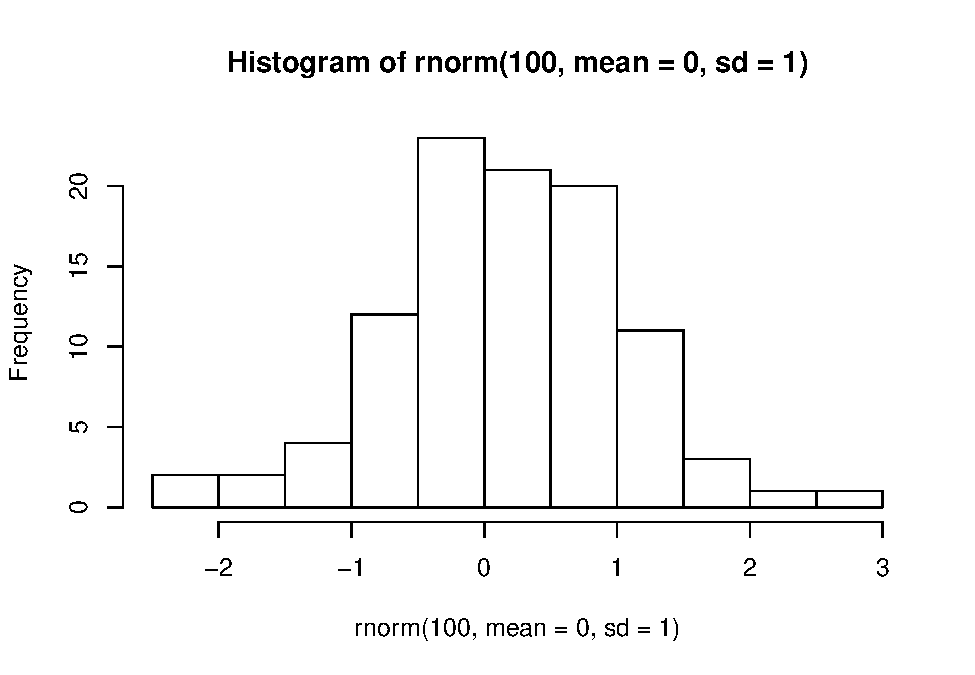
\includegraphics{workshop_notebook_files/figure-latex/unnamed-chunk-8-1.pdf}

Use \texttt{dnorm} for density at a value, \texttt{pnorm} for
distribution function and \texttt{qnorm} for quantile function. Same for
other distributions. Check the help pages for these functions if you're
interested.

\hypertarget{dealing-with-nas}{%
\subsection{Dealing with NAs}\label{dealing-with-nas}}

Identifying and replacing non-available (NA) values in our data sets can
be useful:

\begin{Shaded}
\begin{Highlighting}[]
\NormalTok{v <-}\StringTok{ }\KeywordTok{c}\NormalTok{(}\DecValTok{1}\NormalTok{, }\DecValTok{5}\NormalTok{, }\DecValTok{19}\NormalTok{, }\DecValTok{2}\NormalTok{, }\DecValTok{23}\NormalTok{, }\OtherTok{NA}\NormalTok{, }\DecValTok{3}\NormalTok{, }\DecValTok{9}\NormalTok{, }\OtherTok{NA}\NormalTok{)}
\NormalTok{v}
\end{Highlighting}
\end{Shaded}

\begin{verbatim}
## [1]  1  5 19  2 23 NA  3  9 NA
\end{verbatim}

\begin{Shaded}
\begin{Highlighting}[]
\KeywordTok{is.na}\NormalTok{(v)}
\end{Highlighting}
\end{Shaded}

\begin{verbatim}
## [1] FALSE FALSE FALSE FALSE FALSE  TRUE FALSE FALSE  TRUE
\end{verbatim}

\begin{Shaded}
\begin{Highlighting}[]
\KeywordTok{which}\NormalTok{(}\KeywordTok{is.na}\NormalTok{(v))}
\end{Highlighting}
\end{Shaded}

\begin{verbatim}
## [1] 6 9
\end{verbatim}

\begin{Shaded}
\begin{Highlighting}[]
\CommentTok{# Create a vector without the NAs}
\NormalTok{w <-}\StringTok{ }\NormalTok{v[}\OperatorTok{!}\KeywordTok{is.na}\NormalTok{(v)]}
\NormalTok{w}
\end{Highlighting}
\end{Shaded}

\begin{verbatim}
## [1]  1  5 19  2 23  3  9
\end{verbatim}

\begin{Shaded}
\begin{Highlighting}[]
\CommentTok{# Substitute NAs for e.g. 0}
\NormalTok{v2 <-}\StringTok{ }\NormalTok{v}
\NormalTok{v2[}\KeywordTok{is.na}\NormalTok{(v2)] <-}\StringTok{ }\DecValTok{0}
\NormalTok{v2}
\end{Highlighting}
\end{Shaded}

\begin{verbatim}
## [1]  1  5 19  2 23  0  3  9  0
\end{verbatim}

\begin{Shaded}
\begin{Highlighting}[]
\CommentTok{# Inf (infinite) and NaN (not a number) are different from NA:}
\DecValTok{5}\OperatorTok{/}\DecValTok{0}
\end{Highlighting}
\end{Shaded}

\begin{verbatim}
## [1] Inf
\end{verbatim}

\begin{Shaded}
\begin{Highlighting}[]
\DecValTok{0}\OperatorTok{/}\DecValTok{0}
\end{Highlighting}
\end{Shaded}

\begin{verbatim}
## [1] NaN
\end{verbatim}

\begin{Shaded}
\begin{Highlighting}[]
\KeywordTok{is.infinite}\NormalTok{(}\DecValTok{5}\OperatorTok{/}\DecValTok{0}\NormalTok{)}
\end{Highlighting}
\end{Shaded}

\begin{verbatim}
## [1] TRUE
\end{verbatim}

\begin{Shaded}
\begin{Highlighting}[]
\KeywordTok{is.nan}\NormalTok{(}\DecValTok{0}\OperatorTok{/}\DecValTok{0}\NormalTok{)}
\end{Highlighting}
\end{Shaded}

\begin{verbatim}
## [1] TRUE
\end{verbatim}

\begin{Shaded}
\begin{Highlighting}[]
\CommentTok{# NAs can be removed in some functions}
\KeywordTok{mean}\NormalTok{(v)}
\end{Highlighting}
\end{Shaded}

\begin{verbatim}
## [1] NA
\end{verbatim}

\begin{Shaded}
\begin{Highlighting}[]
\KeywordTok{mean}\NormalTok{(v, }\DataTypeTok{na.rm=}\OtherTok{TRUE}\NormalTok{)}
\end{Highlighting}
\end{Shaded}

\begin{verbatim}
## [1] 8.857143
\end{verbatim}

For linear models (\texttt{lm} function) one can use \texttt{na.omit} or
\texttt{na.exclude}.

\hypertarget{upload-and-exporting}{%
\section{Upload and Exporting}\label{upload-and-exporting}}

\begin{center}\rule{0.5\linewidth}{\linethickness}\end{center}

\hypertarget{importing-data-from-excel}{%
\subsection{Importing data from Excel}\label{importing-data-from-excel}}

To import a data set from Excel the easiest is to save the Excel file as
a comma-separated values (\texttt{.csv}) or a tab-separated values
(\texttt{.tsv}) file.

The \texttt{.csv} and \texttt{.tsv} files can be imported from the tab
``Environment'' in R Studio:

\begin{figure}
\centering
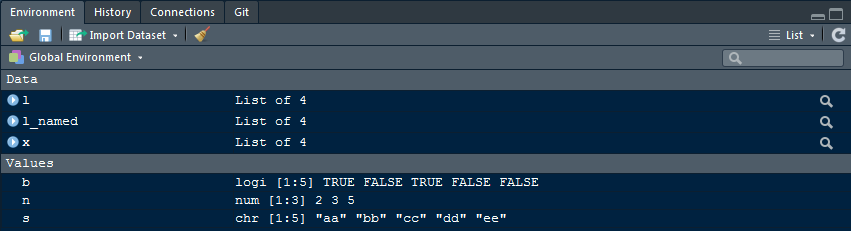
\includegraphics{imgs/Import.PNG}
\caption{Click on \texttt{Import\ Dataset} --\textgreater{}
\texttt{From\ text\ (base)...}.}
\end{figure}

If your data is already organised into columns, tick the box
``Headings''.

Alternatively, you can use the following command:

\begin{Shaded}
\begin{Highlighting}[]
\NormalTok{iris <-}\StringTok{ }\KeywordTok{read.csv}\NormalTok{(}\StringTok{"data/iris.tsv"}\NormalTok{, }\DataTypeTok{header =} \OtherTok{TRUE}\NormalTok{, }\DataTypeTok{sep =} \StringTok{"}\CharTok{\textbackslash{}t}\StringTok{"}\NormalTok{)}
\end{Highlighting}
\end{Shaded}

Check out your data

\begin{Shaded}
\begin{Highlighting}[]
\KeywordTok{head}\NormalTok{(iris)}
\end{Highlighting}
\end{Shaded}

\begin{verbatim}
##   Sepal.Length Sepal.Width Petal.Length Petal.Width Species
## 1          5.1         3.5          1.4         0.2  setosa
## 2          4.9         3.0          1.4         0.2  setosa
## 3          4.7         3.2          1.3         0.2  setosa
## 4          4.6         3.1          1.5         0.2  setosa
## 5          5.0         3.6          1.4         0.2  setosa
## 6          5.4         3.9          1.7         0.4  setosa
\end{verbatim}

\begin{Shaded}
\begin{Highlighting}[]
\KeywordTok{tail}\NormalTok{(iris)}
\end{Highlighting}
\end{Shaded}

\begin{verbatim}
##     Sepal.Length Sepal.Width Petal.Length Petal.Width   Species
## 145          6.7         3.3          5.7         2.5 virginica
## 146          6.7         3.0          5.2         2.3 virginica
## 147          6.3         2.5          5.0         1.9 virginica
## 148          6.5         3.0          5.2         2.0 virginica
## 149          6.2         3.4          5.4         2.3 virginica
## 150          5.9         3.0          5.1         1.8 virginica
\end{verbatim}

\hypertarget{exporting-data}{%
\subsection{Exporting data}\label{exporting-data}}

\begin{Shaded}
\begin{Highlighting}[]
\NormalTok{iris_tail <-}\StringTok{ }\KeywordTok{tail}\NormalTok{(iris)}

\CommentTok{# csv}
\KeywordTok{write.csv}\NormalTok{(iris_tail, }\DataTypeTok{file =} \StringTok{"data/iris_tail.csv"}\NormalTok{, }\DataTypeTok{quote =} \OtherTok{FALSE}\NormalTok{, }\DataTypeTok{row.names =} \OtherTok{FALSE}\NormalTok{, }\DataTypeTok{col.names =} \OtherTok{TRUE}\NormalTok{)}
\end{Highlighting}
\end{Shaded}

\begin{verbatim}
## Warning in write.csv(iris_tail, file = "data/iris_tail.csv", quote = FALSE, :
## attempt to set 'col.names' ignored
\end{verbatim}

\begin{Shaded}
\begin{Highlighting}[]
\CommentTok{# tsv}
\KeywordTok{write.table}\NormalTok{(iris_tail, }\DataTypeTok{file =} \StringTok{"data/iris_tail.tsv"}\NormalTok{, }\DataTypeTok{sep =} \StringTok{"}\CharTok{\textbackslash{}t}\StringTok{"}\NormalTok{, }\DataTypeTok{quote =} \OtherTok{FALSE}\NormalTok{, }\DataTypeTok{row.names =} \OtherTok{FALSE}\NormalTok{, }\DataTypeTok{col.names =} \OtherTok{TRUE}\NormalTok{)}
\end{Highlighting}
\end{Shaded}

\textbf{YOUR TURN \#5} - In the directory ``data'' there is an Excel
file containing a microensor profile that quantified different
parameters. Transform it to \texttt{.csv} format and import it into R.

\hypertarget{installing-packages}{%
\section{Installing Packages}\label{installing-packages}}

\begin{center}\rule{0.5\linewidth}{\linethickness}\end{center}

A package is file containing some functions designed for a specific
task(s). For example, \texttt{ggplot2} is very useful to create elegant
plots and the package \texttt{vegan} is used for ecological analyses.

The package \texttt{readxl} is designed to deal with \texttt{.xlsx}
files. One advantage is that it has functions that allow to read files
with more than one spreadsheet.

Which packages are currently loaded?

\begin{Shaded}
\begin{Highlighting}[]
\KeywordTok{sessionInfo}\NormalTok{()}
\end{Highlighting}
\end{Shaded}

\begin{verbatim}
## R version 3.6.2 (2019-12-12)
## Platform: i386-w64-mingw32/i386 (32-bit)
## Running under: Windows 7 x64 (build 7601) Service Pack 1
## 
## Matrix products: default
## 
## locale:
## [1] LC_COLLATE=German_Germany.1252  LC_CTYPE=German_Germany.1252   
## [3] LC_MONETARY=German_Germany.1252 LC_NUMERIC=C                   
## [5] LC_TIME=German_Germany.1252    
## 
## attached base packages:
## [1] stats     graphics  grDevices utils     datasets  methods   base     
## 
## loaded via a namespace (and not attached):
##  [1] compiler_3.6.2  magrittr_1.5    tools_3.6.2     htmltools_0.4.0
##  [5] yaml_2.2.0      Rcpp_1.0.3      stringi_1.4.4   rmarkdown_2.0  
##  [9] knitr_1.26      stringr_1.4.0   xfun_0.11       digest_0.6.23  
## [13] rlang_0.4.2     evaluate_0.14
\end{verbatim}

To install a package and to activate it in the current workspace we do:

\begin{verbatim}
# To install a package (this task can take a while and may ask for additional packages to be installed):
install.packages("ggplot2")

# To call the package and use its functions in the current session use:
library(ggplot2) # or:
require(ggplot2)
\end{verbatim}

Using the \href{https://bioconductor.org/}{Bioconductor} software to
install packages is highly recommended:

\begin{verbatim}
if (!requireNamespace("BiocManager"))
    install.packages("BiocManager")   # This command installs BiocManager if it is not already installed. 

BiocManager::install("ggplot2")

require(ggplot2)
\end{verbatim}

\hypertarget{tidyverse-packages}{%
\section{Tidyverse packages}\label{tidyverse-packages}}

\begin{center}\rule{0.5\linewidth}{\linethickness}\end{center}

The Tidyverse packages are a modern set of functions that are based on
\href{https://cran.r-project.org/web/packages/tidyverse/vignettes/manifesto.html}{the
tidy tools manifesto} by Hadley Wickham. Two of the principles in the
manifesto that we believe are important for teaching R are:

\begin{itemize}
\tightlist
\item
  Compose simple functions with the pipe
\item
  Designed for humans
\end{itemize}

We will show you how the Tidyverse tools maintain these principles
later.

There have been some
\href{http://varianceexplained.org/r/teach-tidyverse/}{hot debates}
about how to teach R to beginners. The point of contention is whether to
teach students Base R first or go straight to the Tidyverse packages.
David and I believe a balance is really import, so today we will show
you both :)

Here are the tools we will be using today:

\begin{itemize}
\tightlist
\item
  tibble: better data frames
\item
  dplyr: a fast, consistent tool for working with data frame like
  objects
\item
  readr: to import data from files
\item
  tidyr: data tidying and rearrangement
\end{itemize}

To load all these awesome packages at once, run this code

\begin{Shaded}
\begin{Highlighting}[]
\KeywordTok{library}\NormalTok{(tidyverse)}
\end{Highlighting}
\end{Shaded}

\begin{verbatim}
## -- Attaching packages --------------- tidyverse 1.3.0 --
\end{verbatim}

\begin{verbatim}
## v ggplot2 3.2.1     v purrr   0.3.3
## v tibble  2.1.3     v dplyr   0.8.3
## v tidyr   1.0.0     v stringr 1.4.0
## v readr   1.3.1     v forcats 0.4.0
\end{verbatim}

\begin{verbatim}
## -- Conflicts ------------------ tidyverse_conflicts() --
## x dplyr::filter() masks stats::filter()
## x dplyr::lag()    masks stats::lag()
\end{verbatim}

\begin{Shaded}
\begin{Highlighting}[]
\CommentTok{# or you can load individual package}

\KeywordTok{library}\NormalTok{(dplyr)}
\KeywordTok{library}\NormalTok{(readr)}
\end{Highlighting}
\end{Shaded}

\hypertarget{dplyr}{%
\subsubsection{dplyr}\label{dplyr}}

The \href{https://dplyr.tidyverse.org/}{dplyr} package allows you to
interact with data frames and tibbles (a task most biologist will be
doing). The package is easy to learn because it is based around using
verbs to manipulate your data frames. In fact, dplyr is referred to as,
``the grammar of data manipulation.'' Here are the verbs we will learn
about today:

\begin{itemize}
\tightlist
\item
  Select(): return specific columns of a data frame
\item
  Filter(): extract rows of a data frame that meet specified conditions
\item
  Arrange(): order data by row (i.e.~descending order)
\item
  Rename(): rename the title of a column
\item
  Mutate(): add a new column to your data frame
\item
  Summarise(): return summary statistics for your data frame
\item
  Group\_by(): organizes data into specific groups
\end{itemize}

Here are some code examples!

\hypertarget{select}{%
\subsubsection{Select()}\label{select}}

\begin{Shaded}
\begin{Highlighting}[]
\CommentTok{# load the package}
\KeywordTok{library}\NormalTok{(dplyr)}

\CommentTok{# Check out the iris dataset before and after converting it to a tibble!}
\KeywordTok{head}\NormalTok{(iris)}
\end{Highlighting}
\end{Shaded}

\begin{verbatim}
##   Sepal.Length Sepal.Width Petal.Length Petal.Width Species
## 1          5.1         3.5          1.4         0.2  setosa
## 2          4.9         3.0          1.4         0.2  setosa
## 3          4.7         3.2          1.3         0.2  setosa
## 4          4.6         3.1          1.5         0.2  setosa
## 5          5.0         3.6          1.4         0.2  setosa
## 6          5.4         3.9          1.7         0.4  setosa
\end{verbatim}

\begin{Shaded}
\begin{Highlighting}[]
\NormalTok{iris <-}\StringTok{ }\NormalTok{iris }\OperatorTok\StringTok{ }\KeywordTok{as_tibble}\NormalTok{() }\CommentTok{# much better :)}

\CommentTok{# Print iris and select "Sepal.Length"}
\NormalTok{iris }\OperatorTok\StringTok{ }\KeywordTok{select}\NormalTok{(Sepal.Length)}
\end{Highlighting}
\end{Shaded}

\begin{verbatim}
## # A tibble: 150 x 1
##    Sepal.Length
##           <dbl>
##  1          5.1
##  2          4.9
##  3          4.7
##  4          4.6
##  5          5  
##  6          5.4
##  7          4.6
##  8          5  
##  9          4.4
## 10          4.9
## # ... with 140 more rows
\end{verbatim}

Notice the \texttt{\%\textgreater{}\%} symbol, this is known as a pipe.
You can think of it as ``piping'' the output of one command into another
command. By structuring your code this way, it becomes closer to natural
language!

The tibble and the \texttt{\%\textgreater{}\%} are two examples of how
Tidyverse tools and packages use the principles:

\begin{enumerate}
\def\labelenumi{(\arabic{enumi})}
\tightlist
\item
  Compos simple functions with the pipe
\item
  Designed for humans
\end{enumerate}

This code block could be read as, ``Print the iris object then select
the Sepal.Length column''

\begin{Shaded}
\begin{Highlighting}[]
\NormalTok{iris }\OperatorTok\StringTok{ }\KeywordTok{select}\NormalTok{(Sepal.Length)}
\end{Highlighting}
\end{Shaded}

\begin{verbatim}
## # A tibble: 150 x 1
##    Sepal.Length
##           <dbl>
##  1          5.1
##  2          4.9
##  3          4.7
##  4          4.6
##  5          5  
##  6          5.4
##  7          4.6
##  8          5  
##  9          4.4
## 10          4.9
## # ... with 140 more rows
\end{verbatim}

\begin{Shaded}
\begin{Highlighting}[]
\CommentTok{# Try reading Base R to yourself... trust me it won't form a normal sentence ;)}
\end{Highlighting}
\end{Shaded}

Exercise: Import the excel file \texttt{data/titanic3.xls} and select
the \texttt{age} column.

Let's check out some more dplyr verbs

\hypertarget{filter}{%
\subsubsection{Filter()}\label{filter}}

This verb allows you so subset rows of your data.

\begin{Shaded}
\begin{Highlighting}[]
\CommentTok{# Print iris and filter for rows where Sepal.Length is greater than 5.4}
\NormalTok{iris_long_sepels <-}\StringTok{ }\NormalTok{iris }\OperatorTok\StringTok{ }\KeywordTok{filter}\NormalTok{(Sepal.Length }\OperatorTok{>}\StringTok{ }\FloatTok{5.4}\NormalTok{)}

\CommentTok{# Print both of these data frames and take notice of the reduction in dimensions}
\NormalTok{iris}
\end{Highlighting}
\end{Shaded}

\begin{verbatim}
## # A tibble: 150 x 5
##    Sepal.Length Sepal.Width Petal.Length Petal.Width Species
##           <dbl>       <dbl>        <dbl>       <dbl> <fct>  
##  1          5.1         3.5          1.4         0.2 setosa 
##  2          4.9         3            1.4         0.2 setosa 
##  3          4.7         3.2          1.3         0.2 setosa 
##  4          4.6         3.1          1.5         0.2 setosa 
##  5          5           3.6          1.4         0.2 setosa 
##  6          5.4         3.9          1.7         0.4 setosa 
##  7          4.6         3.4          1.4         0.3 setosa 
##  8          5           3.4          1.5         0.2 setosa 
##  9          4.4         2.9          1.4         0.2 setosa 
## 10          4.9         3.1          1.5         0.1 setosa 
## # ... with 140 more rows
\end{verbatim}

\begin{Shaded}
\begin{Highlighting}[]
\NormalTok{iris_long_sepels}
\end{Highlighting}
\end{Shaded}

\begin{verbatim}
## # A tibble: 98 x 5
##    Sepal.Length Sepal.Width Petal.Length Petal.Width Species   
##           <dbl>       <dbl>        <dbl>       <dbl> <fct>     
##  1          5.8         4            1.2         0.2 setosa    
##  2          5.7         4.4          1.5         0.4 setosa    
##  3          5.7         3.8          1.7         0.3 setosa    
##  4          5.5         4.2          1.4         0.2 setosa    
##  5          5.5         3.5          1.3         0.2 setosa    
##  6          7           3.2          4.7         1.4 versicolor
##  7          6.4         3.2          4.5         1.5 versicolor
##  8          6.9         3.1          4.9         1.5 versicolor
##  9          5.5         2.3          4           1.3 versicolor
## 10          6.5         2.8          4.6         1.5 versicolor
## # ... with 88 more rows
\end{verbatim}

\begin{Shaded}
\begin{Highlighting}[]
\CommentTok{# Print iris and filter for rows where the species is setosa}
\NormalTok{iris }\OperatorTok\StringTok{ }\KeywordTok{filter}\NormalTok{(Species }\OperatorTok{==}\StringTok{ "setosa"}\NormalTok{)}
\end{Highlighting}
\end{Shaded}

\begin{verbatim}
## # A tibble: 50 x 5
##    Sepal.Length Sepal.Width Petal.Length Petal.Width Species
##           <dbl>       <dbl>        <dbl>       <dbl> <fct>  
##  1          5.1         3.5          1.4         0.2 setosa 
##  2          4.9         3            1.4         0.2 setosa 
##  3          4.7         3.2          1.3         0.2 setosa 
##  4          4.6         3.1          1.5         0.2 setosa 
##  5          5           3.6          1.4         0.2 setosa 
##  6          5.4         3.9          1.7         0.4 setosa 
##  7          4.6         3.4          1.4         0.3 setosa 
##  8          5           3.4          1.5         0.2 setosa 
##  9          4.4         2.9          1.4         0.2 setosa 
## 10          4.9         3.1          1.5         0.1 setosa 
## # ... with 40 more rows
\end{verbatim}

\hypertarget{arrange}{%
\subsubsection{Arrange()}\label{arrange}}

This verb allows you to order your data by value or alphabetically

\begin{Shaded}
\begin{Highlighting}[]
\CommentTok{# Print iris and arrange the rows from smalled to longest Sepal.Length}
\NormalTok{iris }\OperatorTok\StringTok{ }\KeywordTok{arrange}\NormalTok{(Sepal.Length)}
\end{Highlighting}
\end{Shaded}

\begin{verbatim}
## # A tibble: 150 x 5
##    Sepal.Length Sepal.Width Petal.Length Petal.Width Species
##           <dbl>       <dbl>        <dbl>       <dbl> <fct>  
##  1          4.3         3            1.1         0.1 setosa 
##  2          4.4         2.9          1.4         0.2 setosa 
##  3          4.4         3            1.3         0.2 setosa 
##  4          4.4         3.2          1.3         0.2 setosa 
##  5          4.5         2.3          1.3         0.3 setosa 
##  6          4.6         3.1          1.5         0.2 setosa 
##  7          4.6         3.4          1.4         0.3 setosa 
##  8          4.6         3.6          1           0.2 setosa 
##  9          4.6         3.2          1.4         0.2 setosa 
## 10          4.7         3.2          1.3         0.2 setosa 
## # ... with 140 more rows
\end{verbatim}

\begin{Shaded}
\begin{Highlighting}[]
\CommentTok{# How about descending order!?}
\NormalTok{iris }\OperatorTok\StringTok{ }\KeywordTok{arrange}\NormalTok{(}\KeywordTok{desc}\NormalTok{(Sepal.Length))}
\end{Highlighting}
\end{Shaded}

\begin{verbatim}
## # A tibble: 150 x 5
##    Sepal.Length Sepal.Width Petal.Length Petal.Width Species  
##           <dbl>       <dbl>        <dbl>       <dbl> <fct>    
##  1          7.9         3.8          6.4         2   virginica
##  2          7.7         3.8          6.7         2.2 virginica
##  3          7.7         2.6          6.9         2.3 virginica
##  4          7.7         2.8          6.7         2   virginica
##  5          7.7         3            6.1         2.3 virginica
##  6          7.6         3            6.6         2.1 virginica
##  7          7.4         2.8          6.1         1.9 virginica
##  8          7.3         2.9          6.3         1.8 virginica
##  9          7.2         3.6          6.1         2.5 virginica
## 10          7.2         3.2          6           1.8 virginica
## # ... with 140 more rows
\end{verbatim}

\begin{Shaded}
\begin{Highlighting}[]
\CommentTok{# You can also order alphabetically, here's an example:}

\CommentTok{# Make a list of planets}
\NormalTok{planets <-}\StringTok{ }\KeywordTok{c}\NormalTok{(}\StringTok{"Mercury"}\NormalTok{, }\StringTok{"Venus"}\NormalTok{, }\StringTok{"Earth"}\NormalTok{, }\StringTok{"Mars"}\NormalTok{, }\StringTok{"Jupiter"}\NormalTok{)}

\CommentTok{# Convert it to a tibble}
\NormalTok{planets.tbl <-}\StringTok{ }\NormalTok{planets }\OperatorTok\StringTok{ }\KeywordTok{as_tibble}\NormalTok{()}
\end{Highlighting}
\end{Shaded}

\begin{verbatim}
## Warning: Calling `as_tibble()` on a vector is discouraged, because the behavior is likely to change in the future. Use `tibble::enframe(name = NULL)` instead.
## This warning is displayed once per session.
\end{verbatim}

\begin{Shaded}
\begin{Highlighting}[]
\CommentTok{# check it out}
\NormalTok{planets.tbl}
\end{Highlighting}
\end{Shaded}

\begin{verbatim}
## # A tibble: 5 x 1
##   value  
##   <chr>  
## 1 Mercury
## 2 Venus  
## 3 Earth  
## 4 Mars   
## 5 Jupiter
\end{verbatim}

\begin{Shaded}
\begin{Highlighting}[]
\CommentTok{# Arrange the names alphabetically}
\NormalTok{planets.tbl }\OperatorTok\StringTok{ }\KeywordTok{arrange}\NormalTok{(value)}
\end{Highlighting}
\end{Shaded}

\begin{verbatim}
## # A tibble: 5 x 1
##   value  
##   <chr>  
## 1 Earth  
## 2 Jupiter
## 3 Mars   
## 4 Mercury
## 5 Venus
\end{verbatim}

\hypertarget{rename}{%
\subsubsection{Rename()}\label{rename}}

This allows you to rename columns in your data frame

\begin{Shaded}
\begin{Highlighting}[]
\NormalTok{iris_renamed <-}\StringTok{ }\NormalTok{iris }\OperatorTok\StringTok{ }\KeywordTok{rename}\NormalTok{(}\DataTypeTok{new_name =}\NormalTok{ Sepal.Length)}

\CommentTok{# Check it out!}
\NormalTok{iris_renamed}
\end{Highlighting}
\end{Shaded}

\begin{verbatim}
## # A tibble: 150 x 5
##    new_name Sepal.Width Petal.Length Petal.Width Species
##       <dbl>       <dbl>        <dbl>       <dbl> <fct>  
##  1      5.1         3.5          1.4         0.2 setosa 
##  2      4.9         3            1.4         0.2 setosa 
##  3      4.7         3.2          1.3         0.2 setosa 
##  4      4.6         3.1          1.5         0.2 setosa 
##  5      5           3.6          1.4         0.2 setosa 
##  6      5.4         3.9          1.7         0.4 setosa 
##  7      4.6         3.4          1.4         0.3 setosa 
##  8      5           3.4          1.5         0.2 setosa 
##  9      4.4         2.9          1.4         0.2 setosa 
## 10      4.9         3.1          1.5         0.1 setosa 
## # ... with 140 more rows
\end{verbatim}

\hypertarget{mutate}{%
\subsubsection{Mutate()}\label{mutate}}

This verb allows you to add new columns to your data frame

Let's suppose that the ratio between \texttt{Sepal.Length} and
\texttt{Petal.Length} is important for your study. You can add a column
with this ratio by doing this:

\begin{Shaded}
\begin{Highlighting}[]
\NormalTok{iris }\OperatorTok\StringTok{ }\KeywordTok{mutate}\NormalTok{(}\DataTypeTok{sep_to_ped_ratio =}\NormalTok{ Sepal.Length}\OperatorTok{/}\NormalTok{Petal.Length)}
\end{Highlighting}
\end{Shaded}

\begin{verbatim}
## # A tibble: 150 x 6
##    Sepal.Length Sepal.Width Petal.Length Petal.Width Species sep_to_ped_ratio
##           <dbl>       <dbl>        <dbl>       <dbl> <fct>              <dbl>
##  1          5.1         3.5          1.4         0.2 setosa              3.64
##  2          4.9         3            1.4         0.2 setosa              3.5 
##  3          4.7         3.2          1.3         0.2 setosa              3.62
##  4          4.6         3.1          1.5         0.2 setosa              3.07
##  5          5           3.6          1.4         0.2 setosa              3.57
##  6          5.4         3.9          1.7         0.4 setosa              3.18
##  7          4.6         3.4          1.4         0.3 setosa              3.29
##  8          5           3.4          1.5         0.2 setosa              3.33
##  9          4.4         2.9          1.4         0.2 setosa              3.14
## 10          4.9         3.1          1.5         0.1 setosa              3.27
## # ... with 140 more rows
\end{verbatim}

\hypertarget{summarise}{%
\subsubsection{Summarise}\label{summarise}}

This verb allows you to make summary statistics from your data

\begin{Shaded}
\begin{Highlighting}[]
\CommentTok{# Cacluate the mean Sepal.Length and how many observations there are}
\NormalTok{iris }\OperatorTok\StringTok{ }\KeywordTok{summarise}\NormalTok{(}\DataTypeTok{avg_len =} \KeywordTok{mean}\NormalTok{(Sepal.Length), }\DataTypeTok{n =} \KeywordTok{n}\NormalTok{())}
\end{Highlighting}
\end{Shaded}

\begin{verbatim}
## # A tibble: 1 x 2
##   avg_len     n
##     <dbl> <int>
## 1    5.84   150
\end{verbatim}

\hypertarget{group_by}{%
\subsubsection{Group\_by()}\label{group_by}}

This verb allows you to break up your data into groups. In the iris data
set there are multiple species, we many want to calculate statistics
about the individual species and not the whole data set

\begin{Shaded}
\begin{Highlighting}[]
\CommentTok{# Group by species and calculate the mean Sepal.Width}
\NormalTok{iris }\OperatorTok\StringTok{ }\KeywordTok{group_by}\NormalTok{(Species) }\OperatorTok\StringTok{ }\KeywordTok{summarise}\NormalTok{(}\DataTypeTok{avg_sepal_w =} \KeywordTok{mean}\NormalTok{(Sepal.Width))}
\end{Highlighting}
\end{Shaded}

\begin{verbatim}
## # A tibble: 3 x 2
##   Species    avg_sepal_w
##   <fct>            <dbl>
## 1 setosa            3.43
## 2 versicolor        2.77
## 3 virginica         2.97
\end{verbatim}

\begin{Shaded}
\begin{Highlighting}[]
\CommentTok{# Count how many observations there are per species}
\NormalTok{iris }\OperatorTok\StringTok{ }\KeywordTok{group_by}\NormalTok{(Species) }\OperatorTok\StringTok{ }\KeywordTok{count}\NormalTok{()}
\end{Highlighting}
\end{Shaded}

\begin{verbatim}
## # A tibble: 3 x 2
## # Groups:   Species [3]
##   Species        n
##   <fct>      <int>
## 1 setosa        50
## 2 versicolor    50
## 3 virginica     50
\end{verbatim}

Let's test out our new Tidyverse powers with some practice problems :)

\begin{enumerate}
\def\labelenumi{\arabic{enumi}.}
\item
  Import the excel file \texttt{data/titanic3.xls} and select the
  \texttt{age} column.
\item
  In the iris data set what is the average Sepal.Length per species?
\item
  How many passengers on the titanic were older than 20?
\item
  What is the average age of men and women on the titanic?
\item
  How many passengers survived the sinking of the titanic?
\item
  What age was the oldest person to survive the sinking of the titanic?
\item
  From the iris data set, find the standard deviation of Sepal.Length
  per species then export the resulting data frame as a .tsv file in the
  \texttt{/data/} directory of the R Project
\end{enumerate}

\hypertarget{rstudio-projects}{%
\section{RStudio Projects}\label{rstudio-projects}}

\begin{center}\rule{0.5\linewidth}{\linethickness}\end{center}

The objects created in a R session are shown in the tab ``Environment''.
These objects will not be available if we close the R session unless we
save the work space (however by default you're always asked if you want
to save the current work space upon closing R or R Studio).

A good alternative to not deal with this issue is to create a R project.

\hypertarget{click-on-create-a-project.}{%
\subsubsection{1. Click on ``Create a
project''.}\label{click-on-create-a-project.}}

\begin{figure}
\centering

\includegraphics{imgs/RProject.PNG}
\caption{Click on \texttt{Import\ Dataset} --\textgreater{}
\texttt{From\ text\ (base)...}.}
\end{figure}

\hypertarget{associate-your-r-project-with-a-directory-in-your-computer-new-directory-or-existing-directory.-alternatively-you-can-download-a-repository-from-a-version-control-platform-like-github.}{%
\subsubsection{2. Associate your R project with a directory in your
computer (``New Directory'' or ``Existing Directory''). Alternatively,
you can download a repository from a version control platform like
GitHub.}\label{associate-your-r-project-with-a-directory-in-your-computer-new-directory-or-existing-directory.-alternatively-you-can-download-a-repository-from-a-version-control-platform-like-github.}}

\begin{figure}
\centering
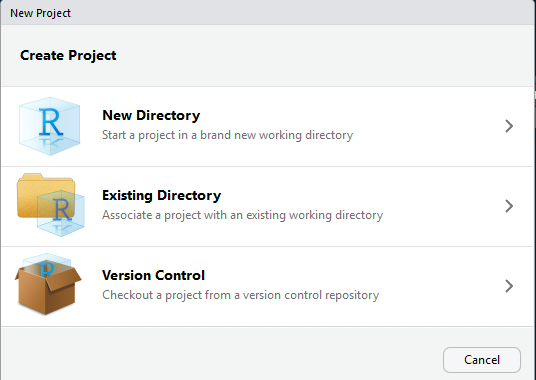
\includegraphics{imgs/RProject1.PNG}
\caption{Click on \texttt{Import\ Dataset} --\textgreater{}
\texttt{From\ text\ (base)...}.}
\end{figure}

\hypertarget{choose-a-name-for-your-directory.-you-can-also-turn-the-directory-into-a-git-repository.}{%
\subsubsection{3. Choose a name for your directory. You can also turn
the directory into a git
repository.}\label{choose-a-name-for-your-directory.-you-can-also-turn-the-directory-into-a-git-repository.}}

\hypertarget{r-markdown-and-r-notebooks}{%
\section{R markdown and R notebooks}\label{r-markdown-and-r-notebooks}}

\begin{center}\rule{0.5\linewidth}{\linethickness}\end{center}

Check the \href{https://www.rstudio.com/resources/cheatsheets/}{R
markdown cheatsheet} for markdown help.

In this section, let's open the file \texttt{workshop\_notebook.Rmd} in
R Studio and check it in parallel to the
\texttt{workshop\_notebook.html} file. We have created a R notebook
(written in R markdown) that can be ``knitted'' to generate the html
document.

The elements of an R Markdown are:

\begin{itemize}
\tightlist
\item
  the header. This is where the title, author, date and output format is
  specified. Output format can be \texttt{.pdf}, \texttt{.html},
  \texttt{.docx}\ldots{}
\item
  the main text. It can include sections, bullet points, tables, etc.
  Sorry to repeat ourselves, but check the
  \href{https://www.rstudio.com/resources/cheatsheets/}{R markdown
  cheatsheet} for more information :)
\item
  code chunks. To insert an R code chunk type
  \texttt{Cntrl}+\texttt{Alt}+\texttt{I} or go to the \texttt{Insert}
  tab in the script window in R Studio. The chunks work like tiny R
  scripts and you can also include comments inside using hash tags (\#).
  Apart from R code, you can include chunks for other coding languages.
\end{itemize}

\hypertarget{credits}{%
\subsection{Credits}\label{credits}}

\begin{center}\rule{0.5\linewidth}{\linethickness}\end{center}

The contents of this workshop were adapted from
\href{http://www.ub.edu/stat/docencia/EADB/Curso\%20basico\%20de\%20R.pdf}{``Curso
básico de R''} by Francesc Carmona, the
\href{https://rawgit.com/genomewalker/p2p/master/friday/P2P_r_crash_course.html\#32_ggplot2}{P2P
course} by Antonio Fernàndez-Guerra and Pelin Yilmaz and
\href{https://astrobiomike.github.io/R/basics}{Happy Belly
Bioinformatics' R basics} by Michael D. Lee.

\hypertarget{contacts}{%
\subsection{Contacts}\label{contacts}}

\begin{center}\rule{0.5\linewidth}{\linethickness}\end{center}

\begin{longtable}[]{@{}lll@{}}
\toprule
Name & GitHub handle & email\tabularnewline
\midrule
\endhead
David Benito & @dbenitom &
\href{mailto:dbenito@mpi-bremen.de}{\nolinkurl{dbenito@mpi-bremen.de}}\tabularnewline
\href{https://orcid.org/0000-0002-8435-3203}{Matthew Schechter} &
@mschecht &
\href{mailto:mschechter@uchicago.edu}{\nolinkurl{mschechter@uchicago.edu}}\tabularnewline
Chiara Vanni & @ChiaraVanni &
\href{mailto:cvanni@mpi-bremen.de}{\nolinkurl{cvanni@mpi-bremen.de}}\tabularnewline
\bottomrule
\end{longtable}

\end{document}
